\documentclass{report}

%%METADATA
\title{Logbook for Fall 2020 Independent Study}
\author{
Luke Motley
}
\date{}

%%PACKAGES
\usepackage{graphicx}
\usepackage{tabularx}
\usepackage{setspace}
\usepackage{amsmath,amsthm,amssymb}
\usepackage[hyphens]{url}
\usepackage{natbib}
\usepackage[font=normalsize,labelfont=bf]{caption}
\usepackage[margin=1in]{geometry}
\usepackage{hyperref}
\hypersetup{colorlinks=true,urlcolor=blue,citecolor=red}
\usepackage{enumerate}% http://ctan.org/pkg/enumerate %Supports lowercase Roman-letter enumeration
\usepackage{verbatim} %Package with \begin{comment} environment
\usepackage{physics}
\usepackage{lscape}
\usepackage{tikz}
\usepackage{tikz-3dplot}
\usepackage{tkz-euclide}
\usepackage{pgfplots}
\pgfplotsset{compat = newest}
\usetikzlibrary{automata,positioning}
\usepgfplotslibrary{external}
\tikzexternalize
\usetikzlibrary{calc,math}
\usepackage{listings}
\usepackage{ulem}
\usepackage{upquote}
\usepackage{booktabs} %Package with \toprule and \bottomrule
\usepackage{etoc}     %Package with \localtableofcontents
\usepackage{multicol}
\usepackage{bm}
\usepackage{placeins} %Package with \FloatBarrier
\setlength{\parskip}{0.5em}
\usepackage{subcaption}
\captionsetup{compatibility=false}
\newcommand{\sym}[1]{\rlap{#1}}% Thanks to David Carlisle

\definecolor{dkgreen}{rgb}{0,0.6,0}
\definecolor{gray}{rgb}{0.5,0.5,0.5}
\definecolor{mauve}{rgb}{0.58,0,0.82}

\lstset{language=bash,
  frame=tb,
  aboveskip=3mm,
  belowskip=3mm,
  showstringspaces=false,
  columns=flexible,
  basicstyle={\small\ttfamily},
  numbers=none,
  numberstyle=\tiny\color{gray},
  keywordstyle=\color{blue},
  commentstyle=\color{dkgreen},
  stringstyle=\color{mauve},
  breaklines=true,
  breakatwhitespace=false,
  tabsize=3
}

\input{entries/listings-stata.tex}   %From https://gist.github.com/mcaceresb/b40d6059cf66cc73423f4ddf3f72acda

%%FORMATTING
\onehalfspacing
\numberwithin{equation}{section}
\numberwithin{figure}{section}
\numberwithin{table}{section}
% \bibliographystyle{../bib/aea}

\newtheorem{observation}{Observation}

%LOGBOOK
\begin{document}

%%LOGBOOK COVER
\maketitle

%TABLE OF CONTENTS
\renewcommand{\thechapter}{\Alph{chapter}}
\setcounter{tocdepth}{2}
\tableofcontents
\etocsettocstyle{}{} % from now on only local tocs

%%LOGBOOK ENTRIES: Related literature
\chapter{Motivation}
\begin{figure}
  \caption{Search Intensity}
    \centering
    \begin{subfigure}[t]{0.5\textwidth}
    \caption{School-centered}
        \centering
        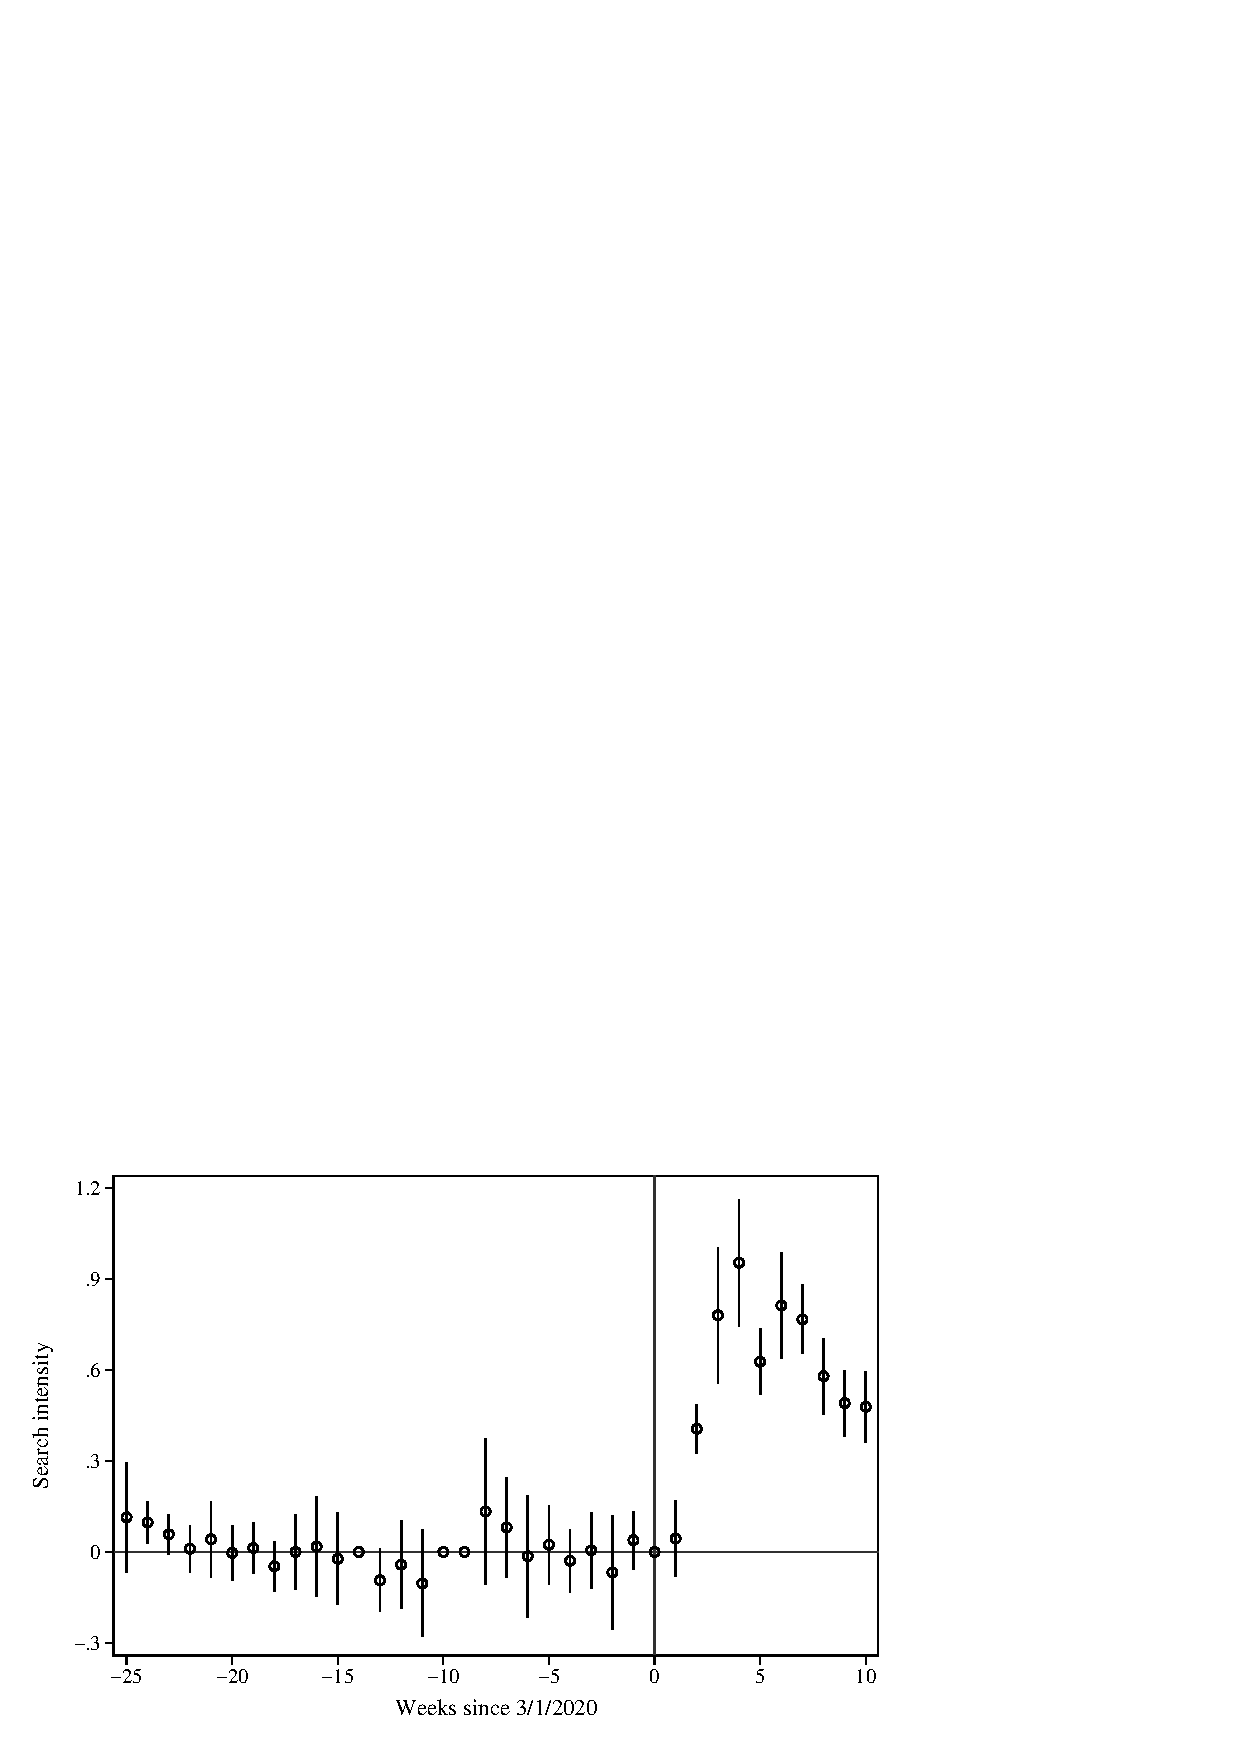
\includegraphics[width=\linewidth]{input/intensity_bh_replication_event_study_specific1.png}
    \end{subfigure}%
    ~
    \begin{subfigure}[t]{0.5\textwidth}
    \caption{Parent-centered}
        \centering
        \includegraphics[width=\linewidth]{input/intensity_bh_replication_event_study_generic.png}
    \end{subfigure}
\end{figure}

\begin{figure}
  \caption{High-Low SES Search Intensity Gap}
    \centering
    \begin{subfigure}[t]{0.5\textwidth}
    \caption{School-centered}
        \centering
        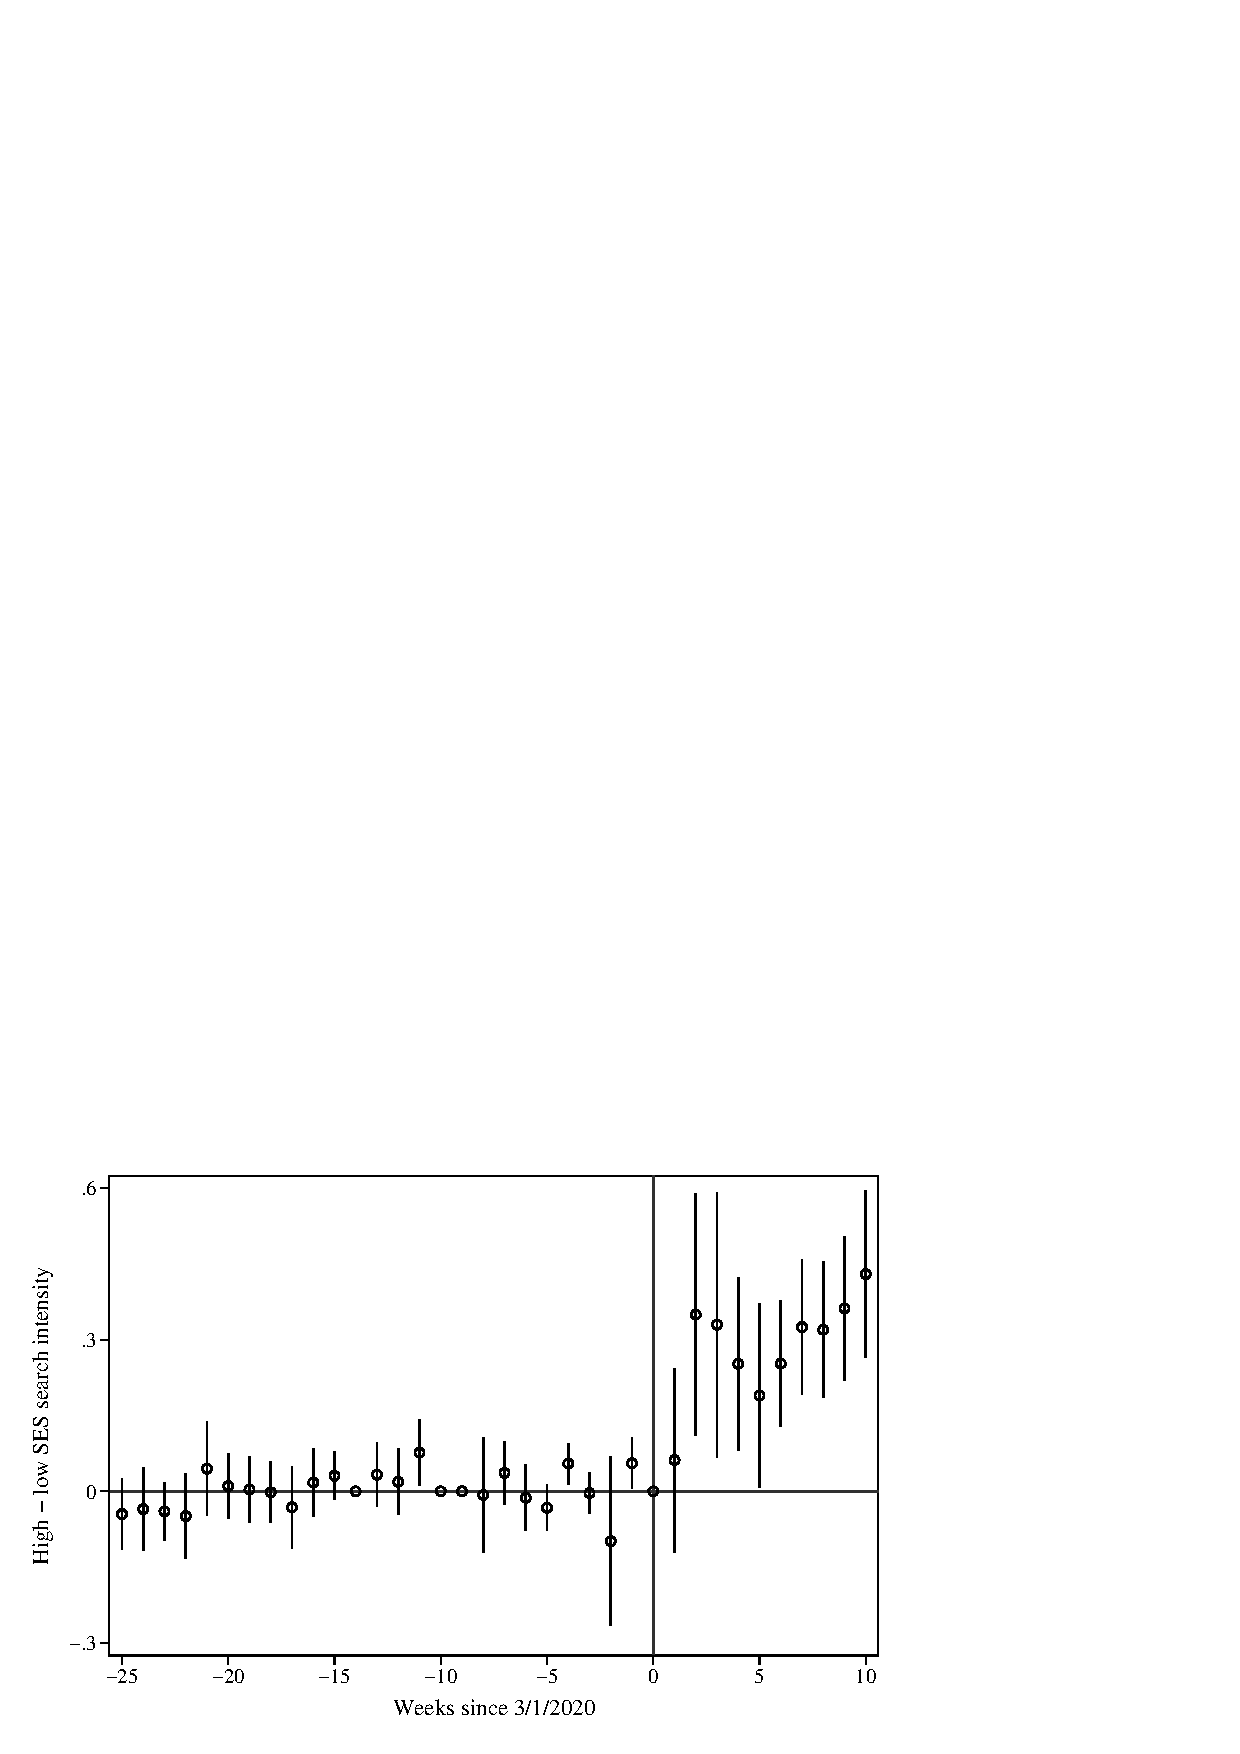
\includegraphics[width=\linewidth]{input/ses_bh_replication_event_study_specific1.png}
    \end{subfigure}%
    ~
    \begin{subfigure}[t]{0.5\textwidth}
    \caption{Parent-centered}
        \centering
        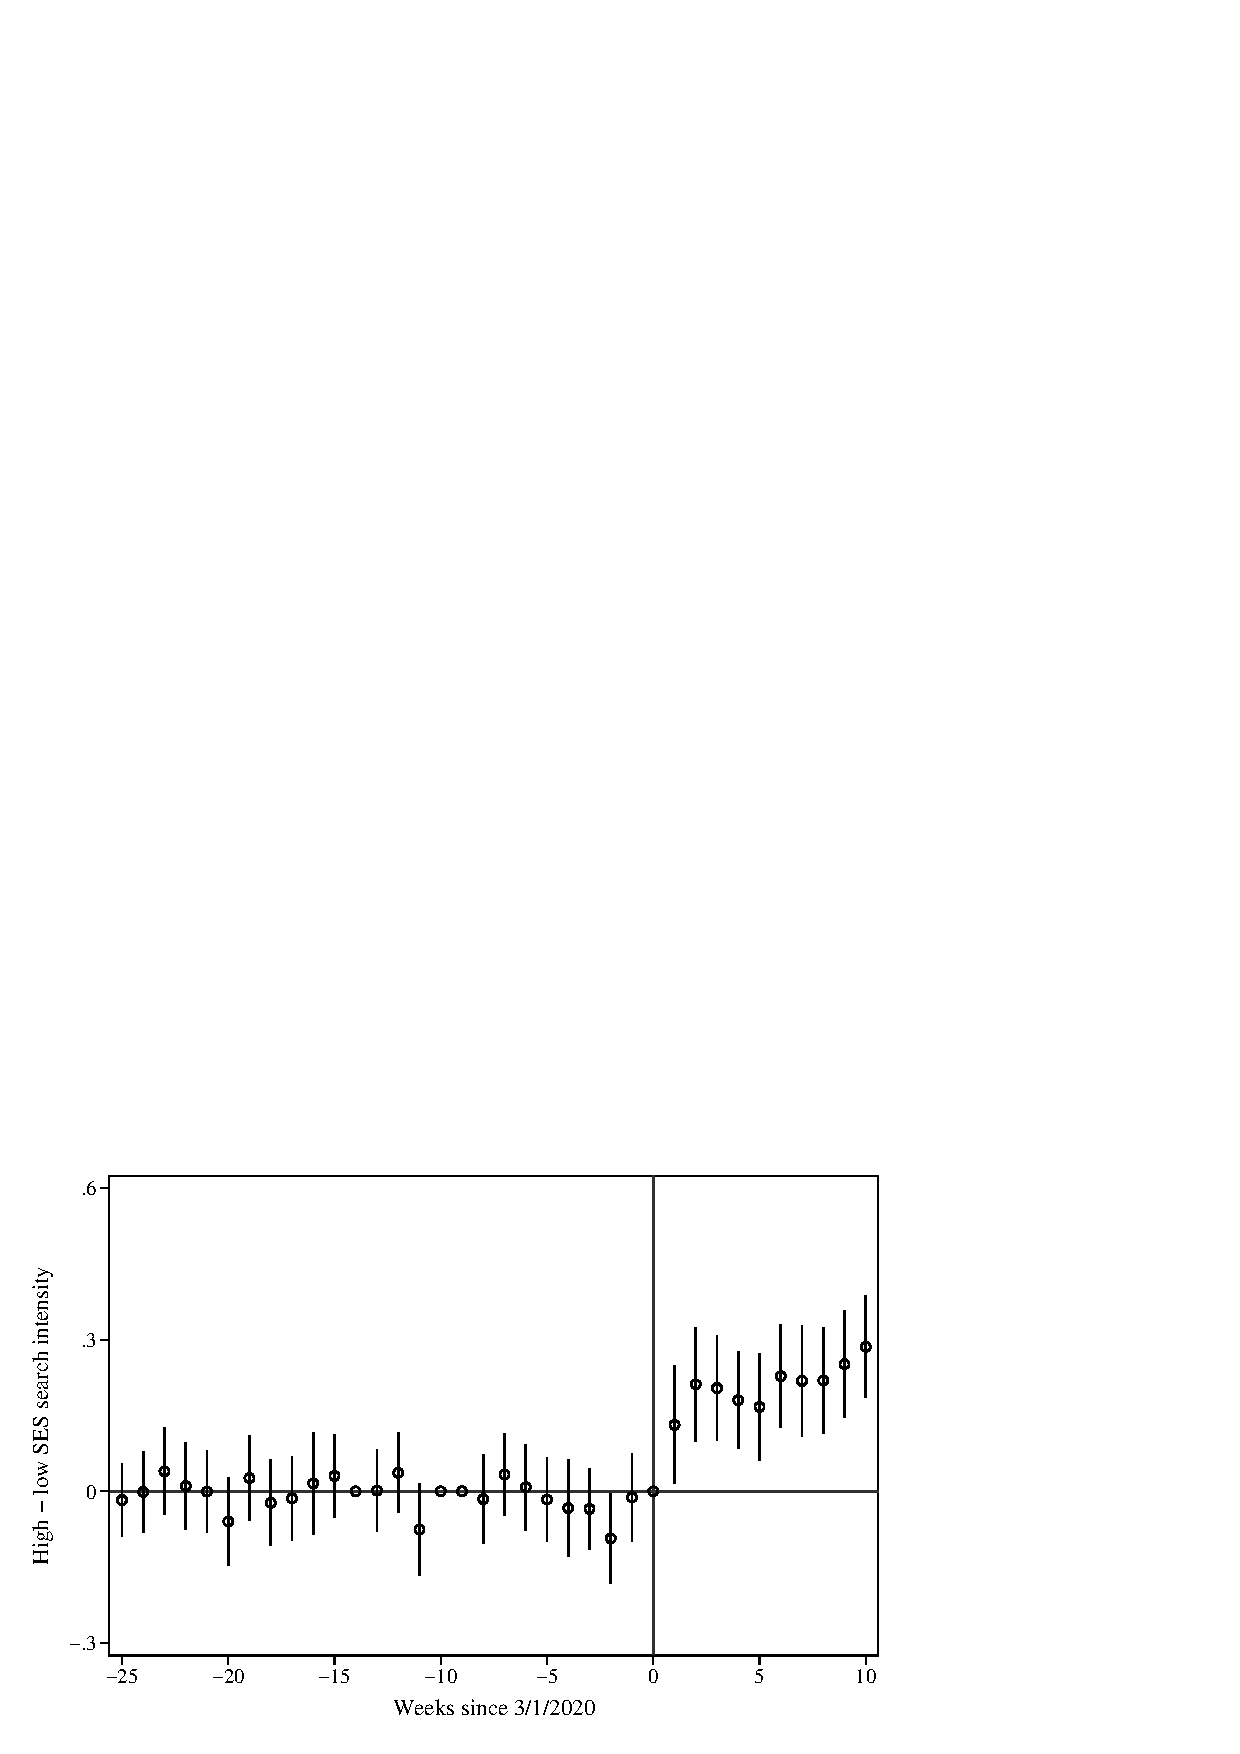
\includegraphics[width=\linewidth]{input/ses_bh_replication_event_study_generic.png}
    \end{subfigure}
\end{figure}

\begin{table}[htbp] \centering
\def\sym#1{\ifmmode^{#1}\else\(^{#1}\)\fi}
\caption{\cite{bh1} Replication: Changes in Search Intensity, excluding low search intensity observations}
\scalebox{0.8}{
\begin{tabular*}{1\textwidth}{@{\extracolsep{\fill}}l*{4}{c}}
\midrule
&School-       &Parent-        &                       &               \\
&centered      &centered       &Google         &Khan   \\
&resources     &resources      &Classroom      &Academy\\
&(1)&(2)&(3)&(4)\\
\midrule
(A) Nationwide \\
\cmidrule{1-1}
Post COVID        &        0.52\sym{***}&        0.35\sym{***}&        0.76\sym{***}&        0.41\sym{***}\\
                    &      (0.05)         &      (0.02)         &      (0.05)         &      (0.03)         \\
\cmidrule{1-1}
(B) By median SES\\
\cmidrule{1-1}
Post COVID $\times$ Low-SES&        0.30\sym{***}&        0.21\sym{***}&        0.59\sym{***}&        0.30\sym{***}\\
                    &      (0.05)         &      (0.02)         &      (0.07)         &      (0.03)         \\
High SES            &       -0.04         &       -0.12\sym{***}&        0.07         &        0.01         \\
                    &      (0.06)         &      (0.03)         &      (0.10)         &      (0.06)         \\
Post COVID $\times$ High-SES&        0.44\sym{***}&        0.27\sym{***}&        0.35\sym{***}&        0.21\sym{***}\\
                    &      (0.10)         &      (0.03)         &      (0.11)         &      (0.05)         \\
                    &                     &                     &                     &                     \\
\cmidrule{1-1}
(C) By income, online access, race\\
\cmidrule{1-1}
Post COVID $\times$ HH mean income&        0.15\sym{***}&        0.09\sym{***}&        0.13\sym{***}&        0.08\sym{***}\\
                    &      (0.03)         &      (0.01)         &      (0.03)         &      (0.02)         \\
                    &                     &                     &                     &                     \\
Post COVID $\times$ \% of HH w/ broadband&        0.43\sym{***}&        0.34\sym{***}&        0.36\sym{***}&        0.30\sym{***}\\
                    &      (0.08)         &      (0.03)         &      (0.09)         &      (0.05)         \\
                    &                     &                     &                     &                     \\
Post COVID $\times$ \% of HH w/ computer&        0.54\sym{***}&        0.46\sym{***}&        0.47\sym{***}&        0.38\sym{***}\\
                    &      (0.10)         &      (0.04)         &      (0.10)         &      (0.07)         \\
                    &                     &                     &                     &                     \\
Post COVID $\times$ \% of schools in rural area&       -0.18\sym{***}&       -0.10\sym{***}&       -0.19\sym{***}&       -0.10\sym{***}\\
                    &      (0.03)         &      (0.01)         &      (0.03)         &      (0.02)         \\
                    &                     &                     &                     &                     \\
Post COVID $\times$ \% of students Black&       -0.09\sym{***}&       -0.04\sym{***}&       -0.02         &       -0.06\sym{***}\\
                    &      (0.03)         &      (0.02)         &      (0.04)         &      (0.02)         \\
                    &                     &                     &                     &                     \\
\hline
& 45845 & 40829 & 45682 & 44240
\end{tabular*}
}
\begin{minipage}{\textwidth}
\footnotesize    \textit{Note:} This replicates DMA-level regressions from \cite{bh1}. The outcomes are in log Google Trends search interest, where (1) and (2) are groupings of terms and (3) and (4) are specific terms. Post-COVID is after March 1, 2020. Panel (A) reveals that COVID-19 is a shock to search interest for resources. Panel (B) shows the results is a difference in differences regression on high-low SES, defined by the median. Panel (C) regresses on each of the individual factors that contribute to SES.
\end{minipage}
\end{table}

\input{input/bh_replication_event_study_table_zero_one.tex}
   
\begin{table}
  \centering
\begin{tabular}{l >{\centering\arraybackslash}m{.15\textwidth} >{\centering\arraybackslash}m{.15\textwidth} >{\centering\arraybackslash}m{.15\textwidth} >{\centering\arraybackslash}m{.15\textwidth}}
    \toprule
                        &\multicolumn{1}{c}{specific1}&\multicolumn{1}{c}{generic}&\multicolumn{1}{c}{engagement}&\multicolumn{1}{c}{badges}\\
[1em]
 \\
    \midrule
    [1em]
Post Covid=1        &       0.473\sym{***}&       0.369\sym{***}&       0.168\sym{**} &       0.168\sym{**} \\
                    &      (9.76)         &     (14.48)         &      (3.26)         &      (3.26)         \\
 \\
    \midrule \\
    [1em]
Post Covid=1        &      -6.931\sym{***}&      -4.251\sym{***}&      -3.023\sym{*}  &      -3.023\sym{*}  \\
                    &     (-5.37)         &     (-7.44)         &     (-2.51)         &     (-2.51)         \\
[1em]
Post Covid=1 $\times$ Log Income&       0.666\sym{***}&       0.415\sym{***}&       0.287\sym{*}  &       0.287\sym{*}  \\
                    &      (5.68)         &      (8.11)         &      (2.63)         &      (2.63)         \\
 \\
    \midrule \\
    [1em]
Post Covid=1        &       1.486\sym{***}&       0.967\sym{***}&       0.396\sym{*}  &       0.396\sym{*}  \\
                    &      (4.68)         &     (14.69)         &      (2.08)         &      (2.08)         \\
[1em]
Post Covid=1 $\times$ Log Teleworkability&       1.009\sym{**} &       0.597\sym{***}&       0.228         &       0.228         \\
                    &      (3.52)         &      (8.85)         &      (1.35)         &      (1.35)         \\
 \\
    \midrule \\
    [1em]
Post Covid=1        &      -4.082\sym{*}  &      -2.737\sym{**} &      -3.389\sym{*}  &      -3.389\sym{*}  \\
                    &     (-2.20)         &     (-3.14)         &     (-2.52)         &     (-2.52)         \\
[1em]
Post Covid=1 $\times$ Log Income&       0.460\sym{**} &       0.306\sym{***}&       0.313\sym{**} &       0.313\sym{**} \\
                    &      (3.21)         &      (4.32)         &      (2.75)         &      (2.75)         \\
[1em]
Post Covid=1 $\times$ Log Teleworkability&       0.564         &       0.300\sym{**} &     -0.0722         &     -0.0722         \\
                    &      (1.59)         &      (2.97)         &     (-0.40)         &     (-0.40)         \\
 \\
    \midrule \\
    [1em]
[1em]
Observations        &      275757         &      263070         &       79227         &       79227         \\
 \\
    \bottomrule
  \end{tabular}
\end{table}

\begin{figure}
  \caption{School-Centered Resources}
    \centering
    \begin{subfigure}[t]{0.45\textwidth}
    \caption{Intensity}
        \centering
        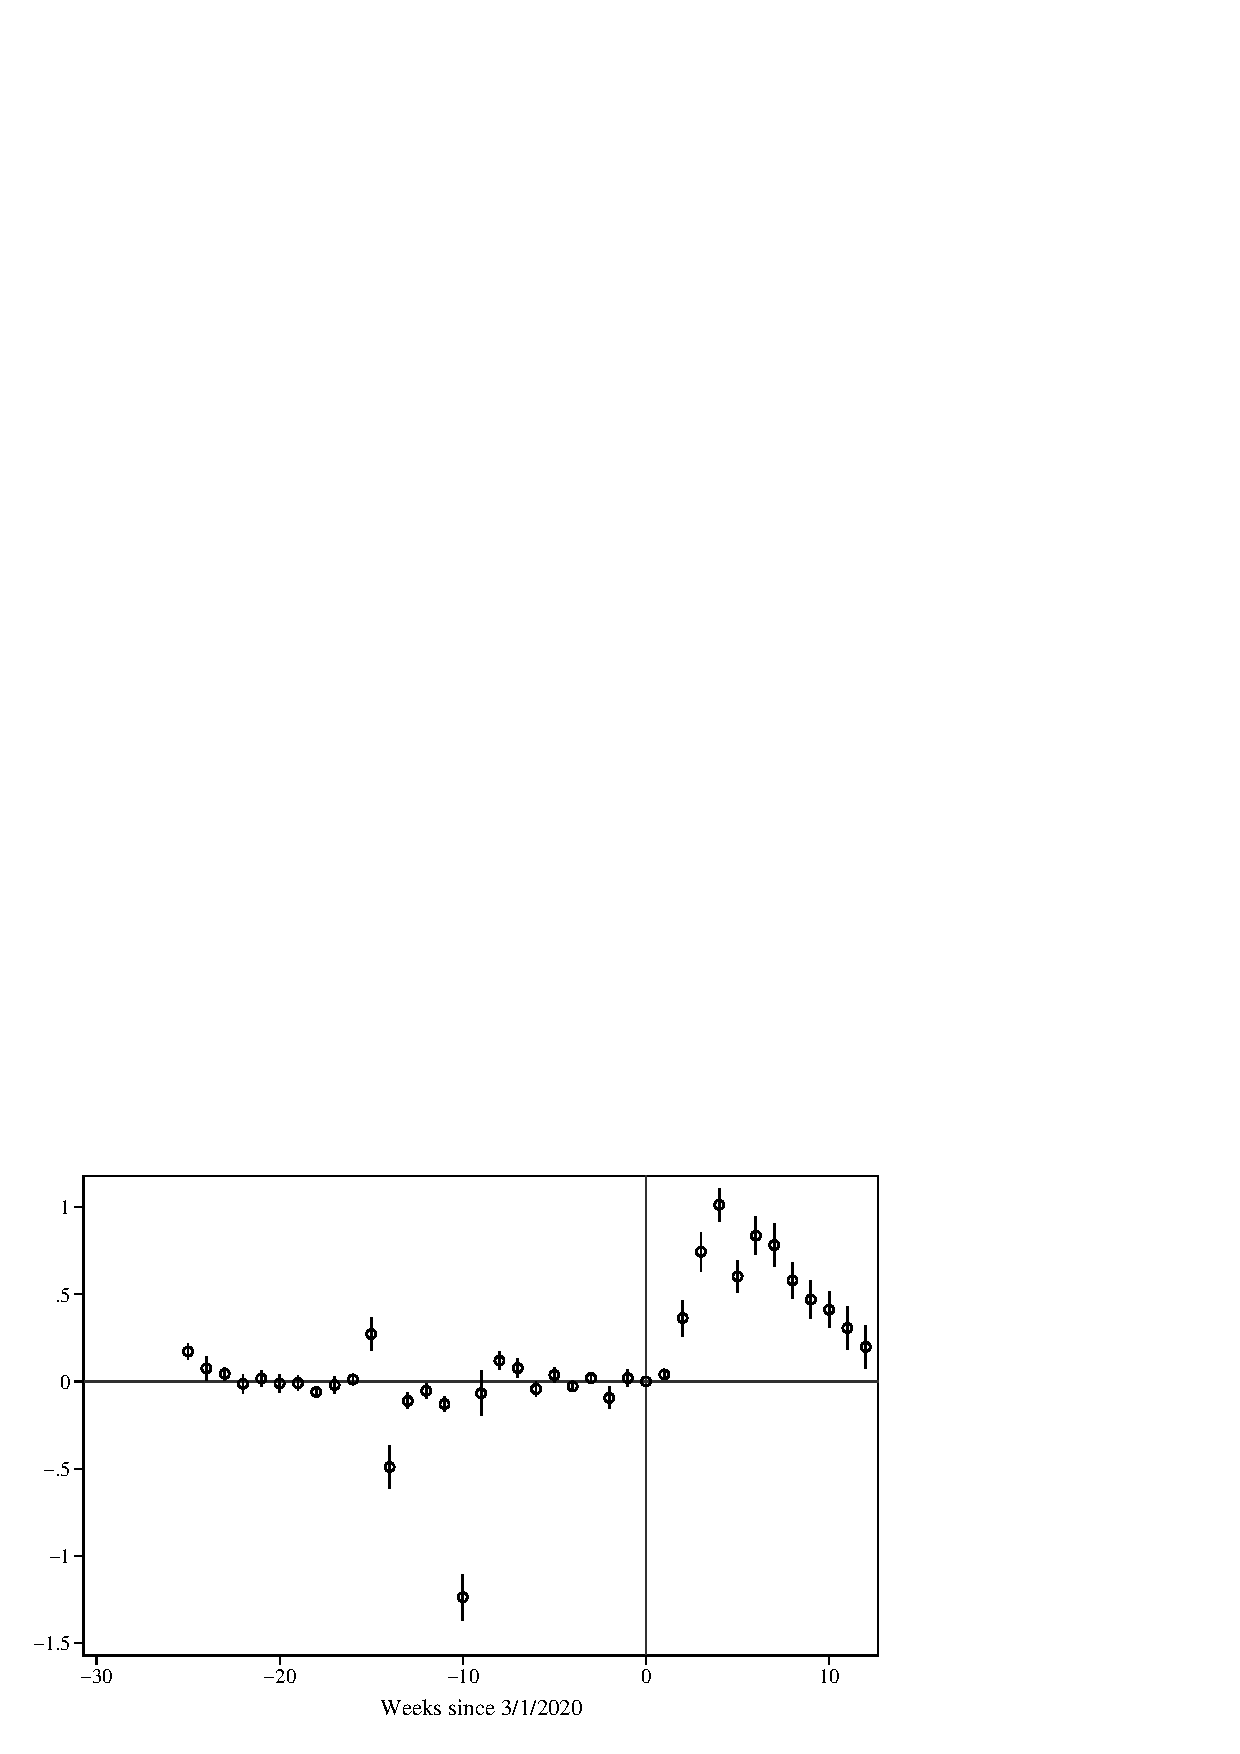
\includegraphics[width=\linewidth]{input/event_study_specific1_wks.png}
    \end{subfigure}%
    \begin{subfigure}[t]{0.45\textwidth}
    \caption{Income}
        \centering
        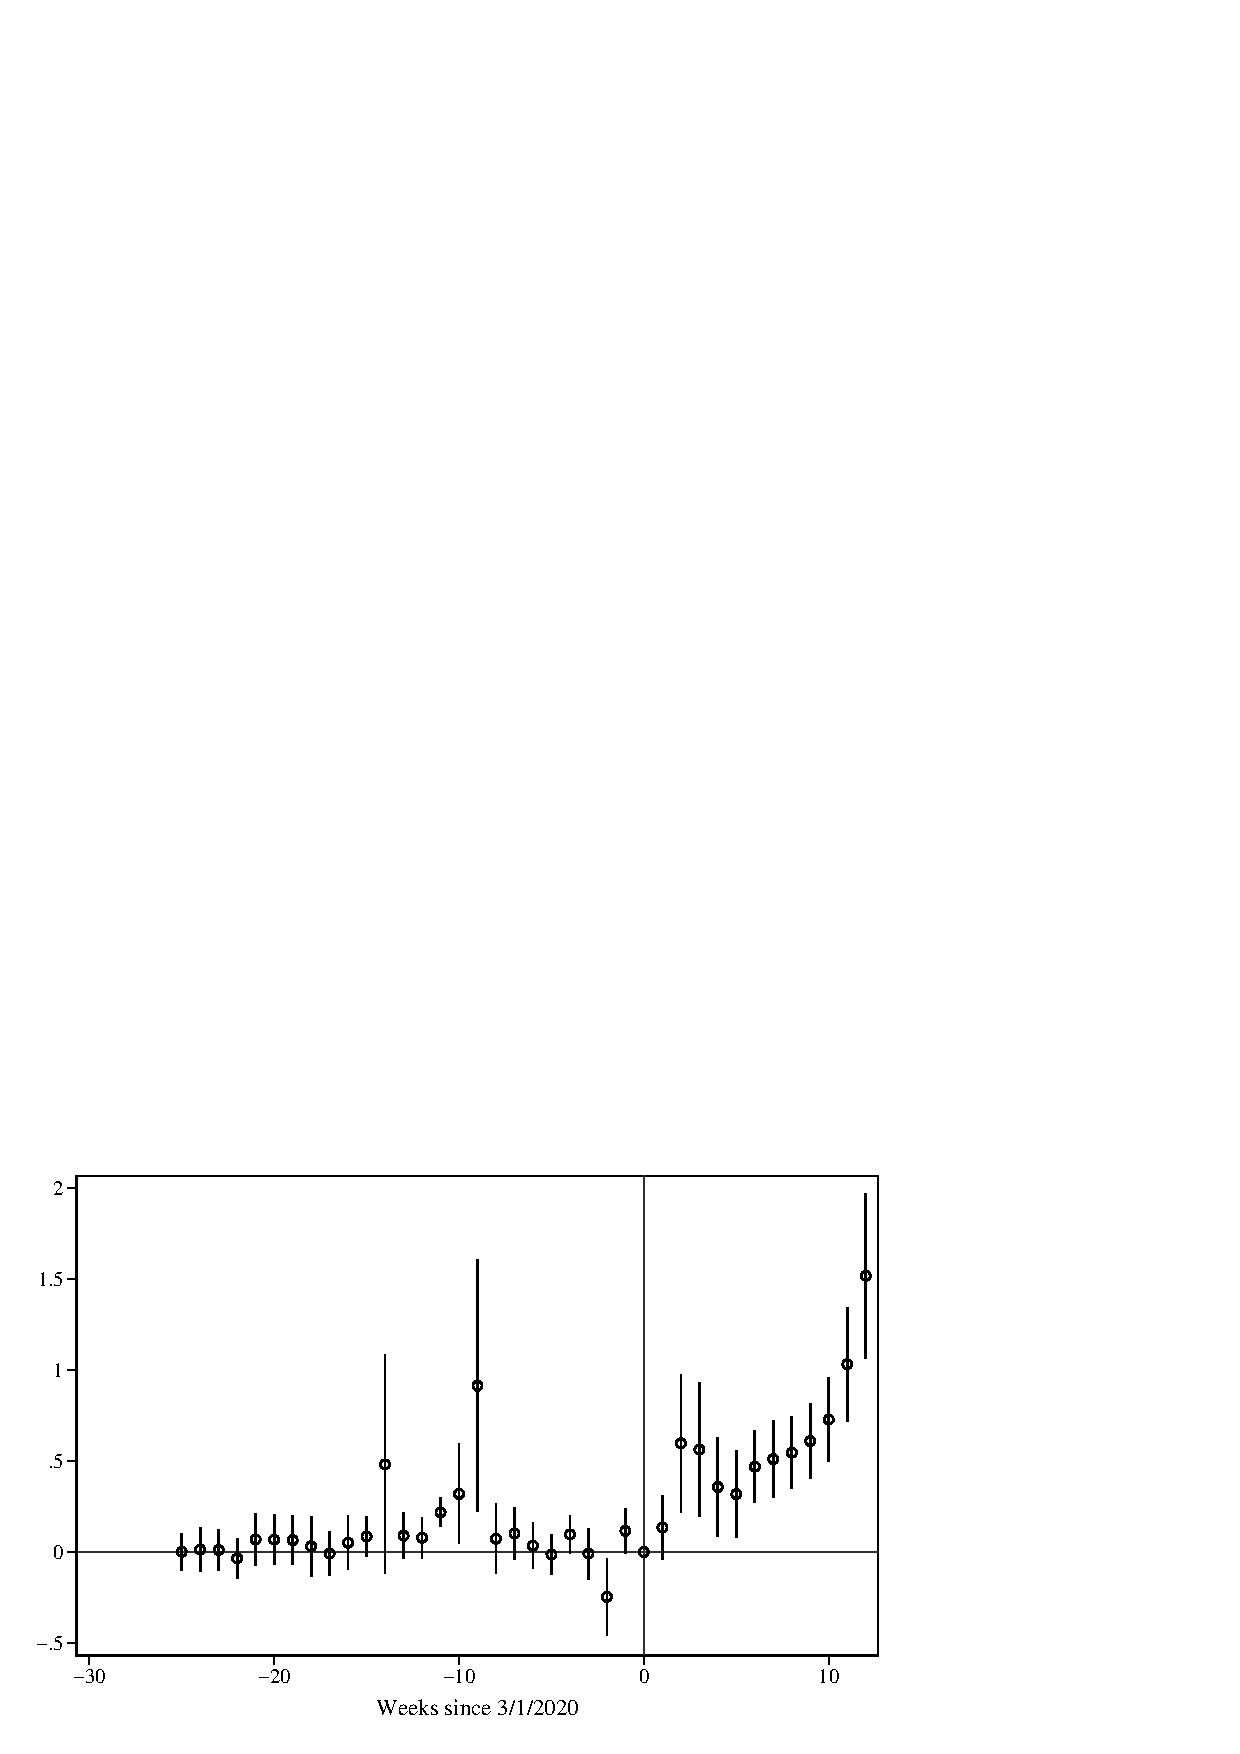
\includegraphics[width=\linewidth]{input/event_study_specific1_inc.png}
    \end{subfigure}%

    \begin{subfigure}{0.45\textwidth}
    \caption{Teleworkability}
        \centering
        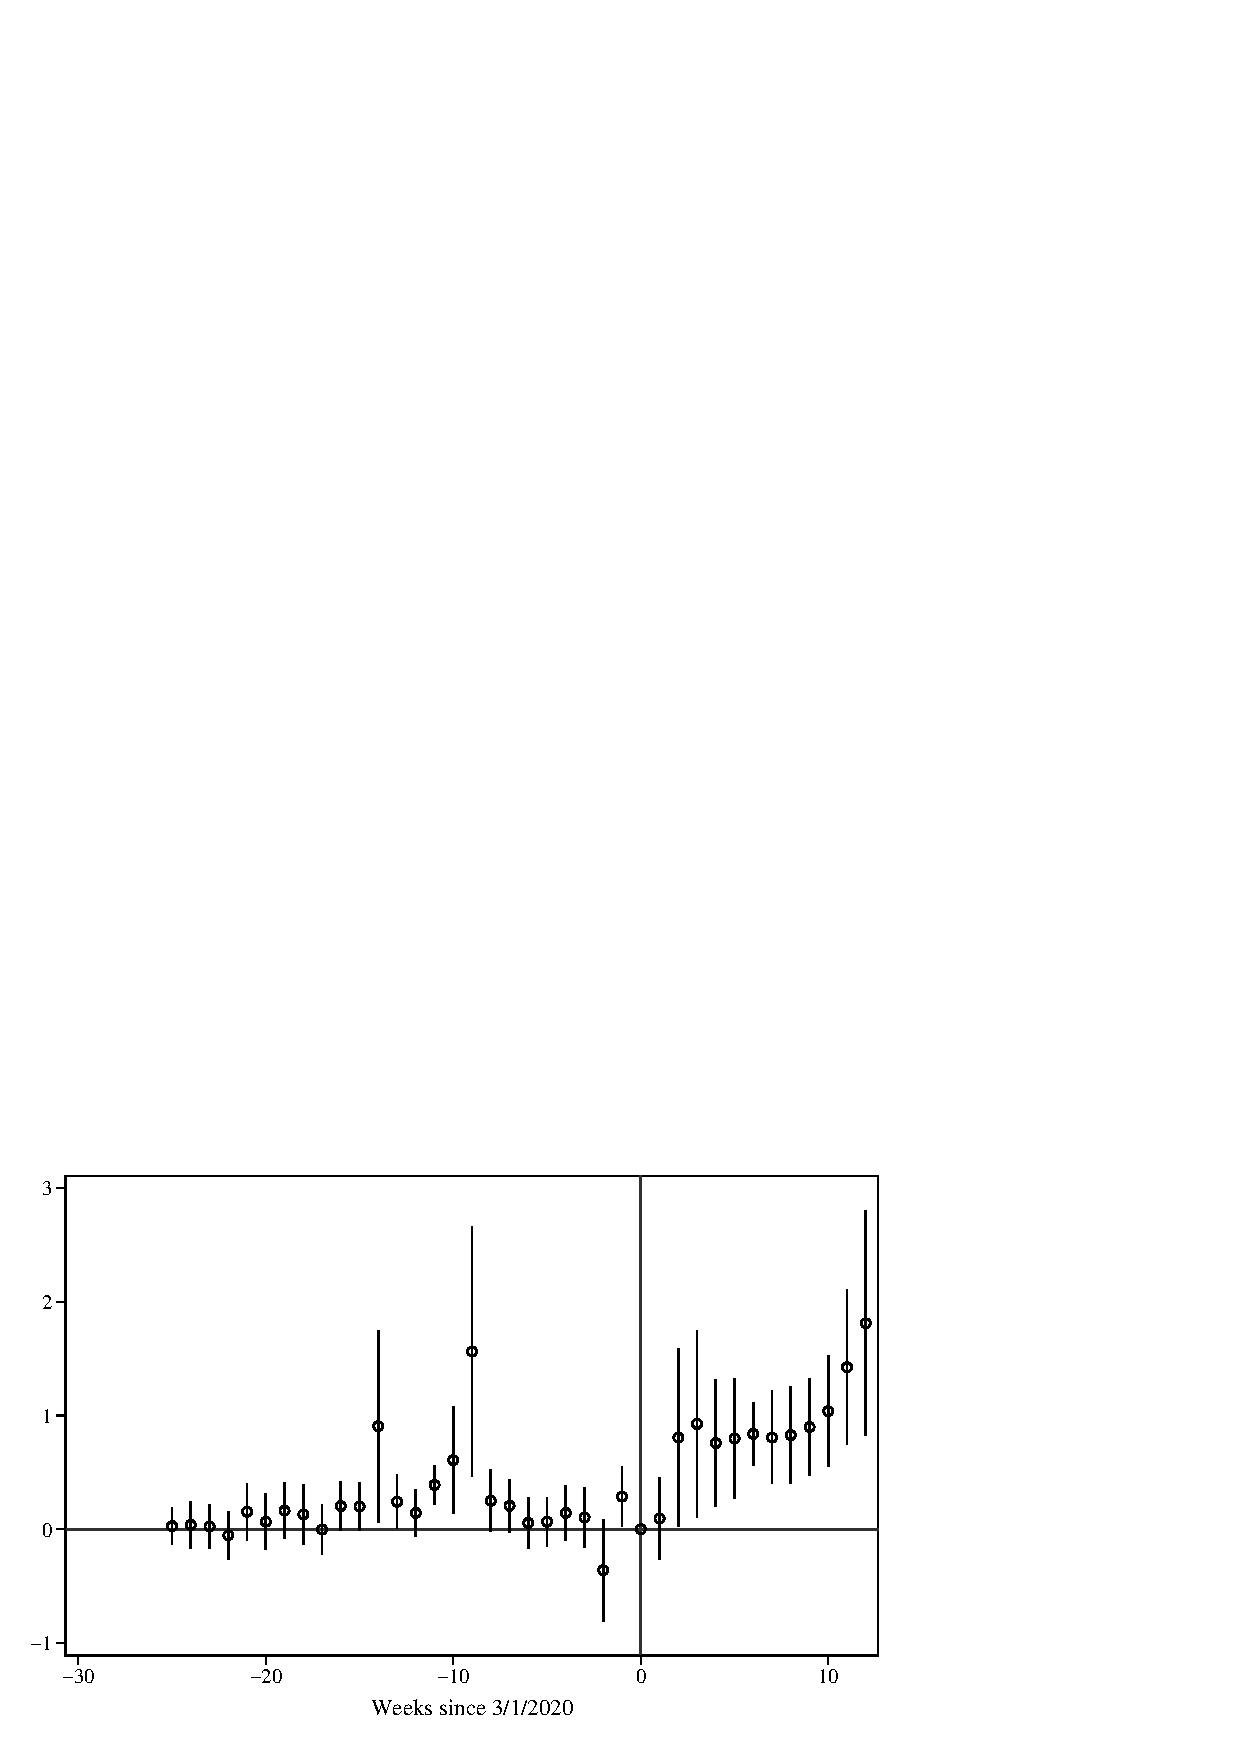
\includegraphics[width=\linewidth]{input/event_study_specific1_tele.png}
    \end{subfigure}%
    \begin{subfigure}{0.45\textwidth}
    \caption{Income + Teleworkability}
        \centering
        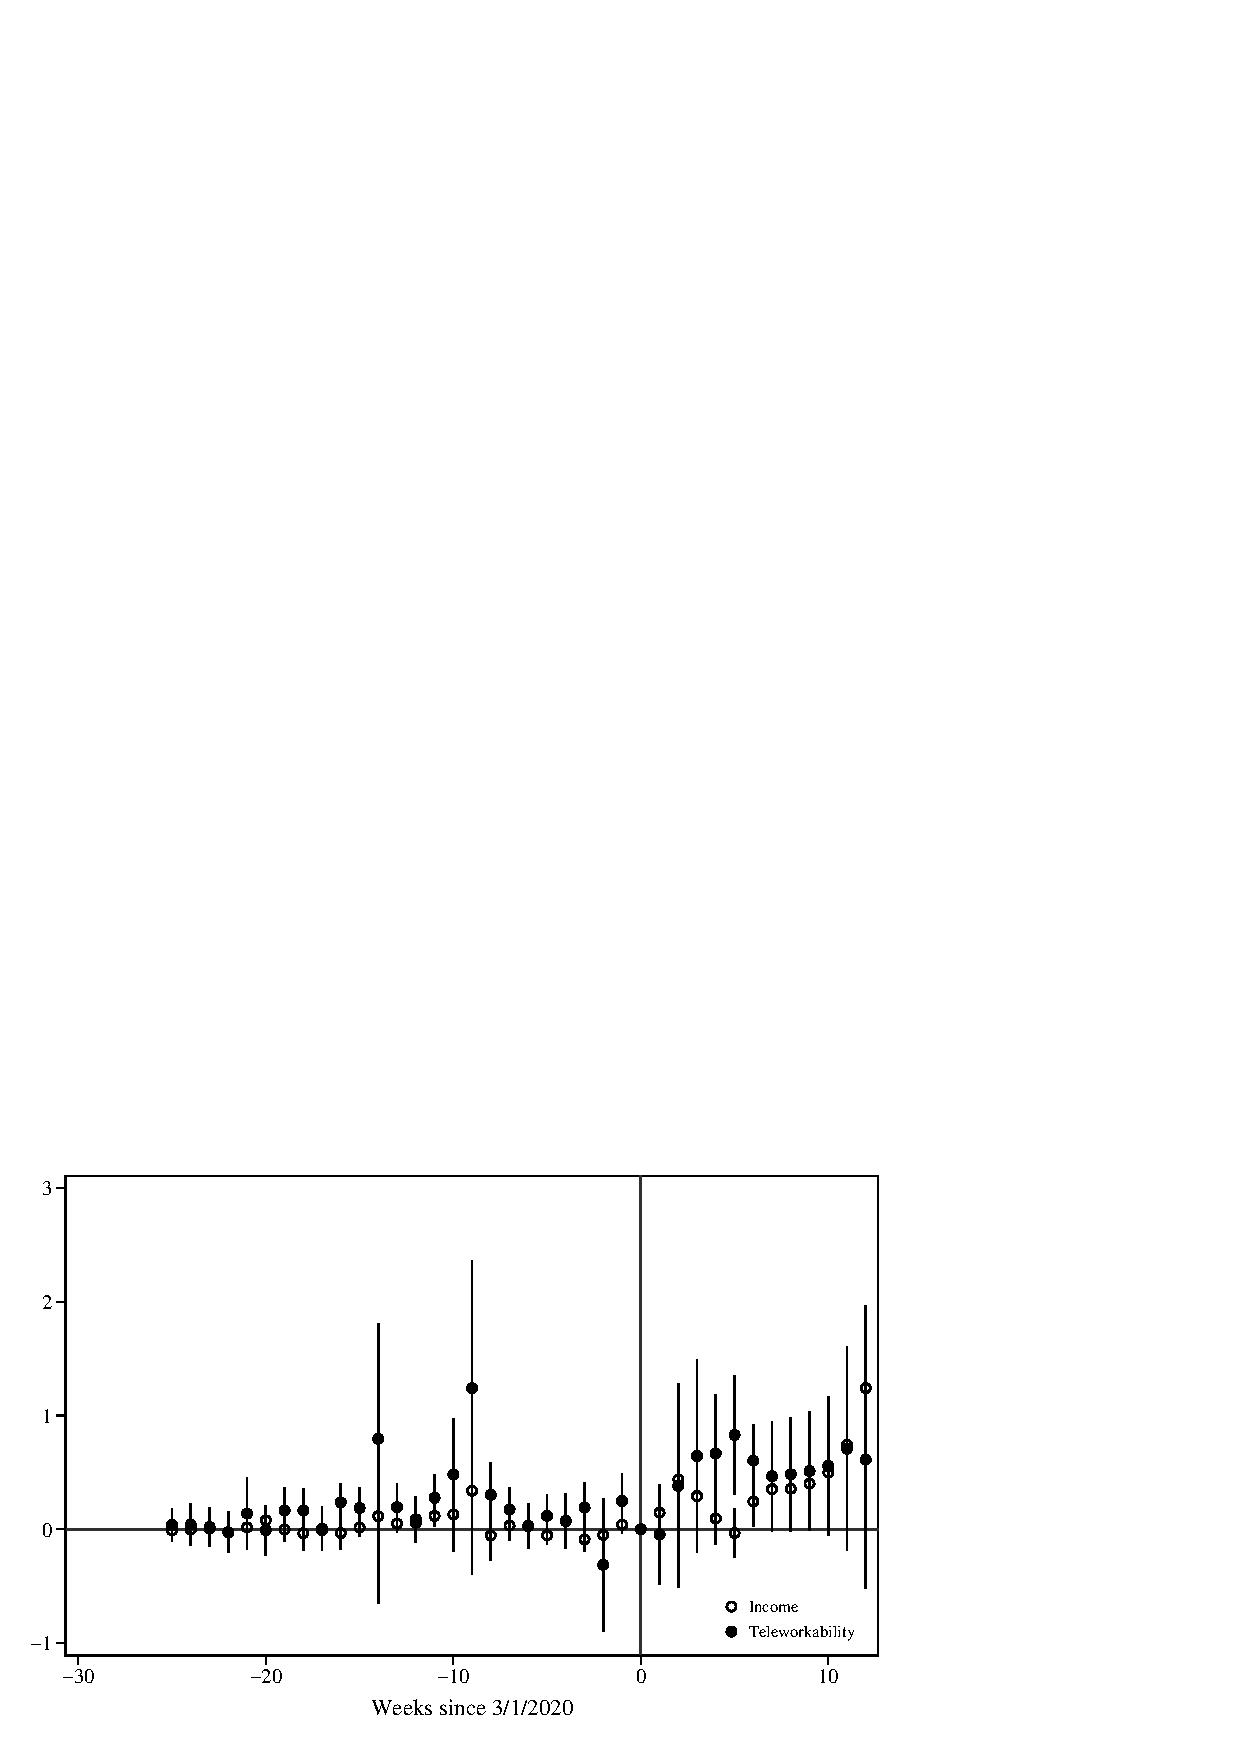
\includegraphics[width=\linewidth]{input/event_study_specific1_inctele.png}
    \end{subfigure}%

  \caption{Parent-Centered}
    \centering
    \begin{subfigure}[t]{0.45\textwidth}
    \caption{Intensity}
        \centering
        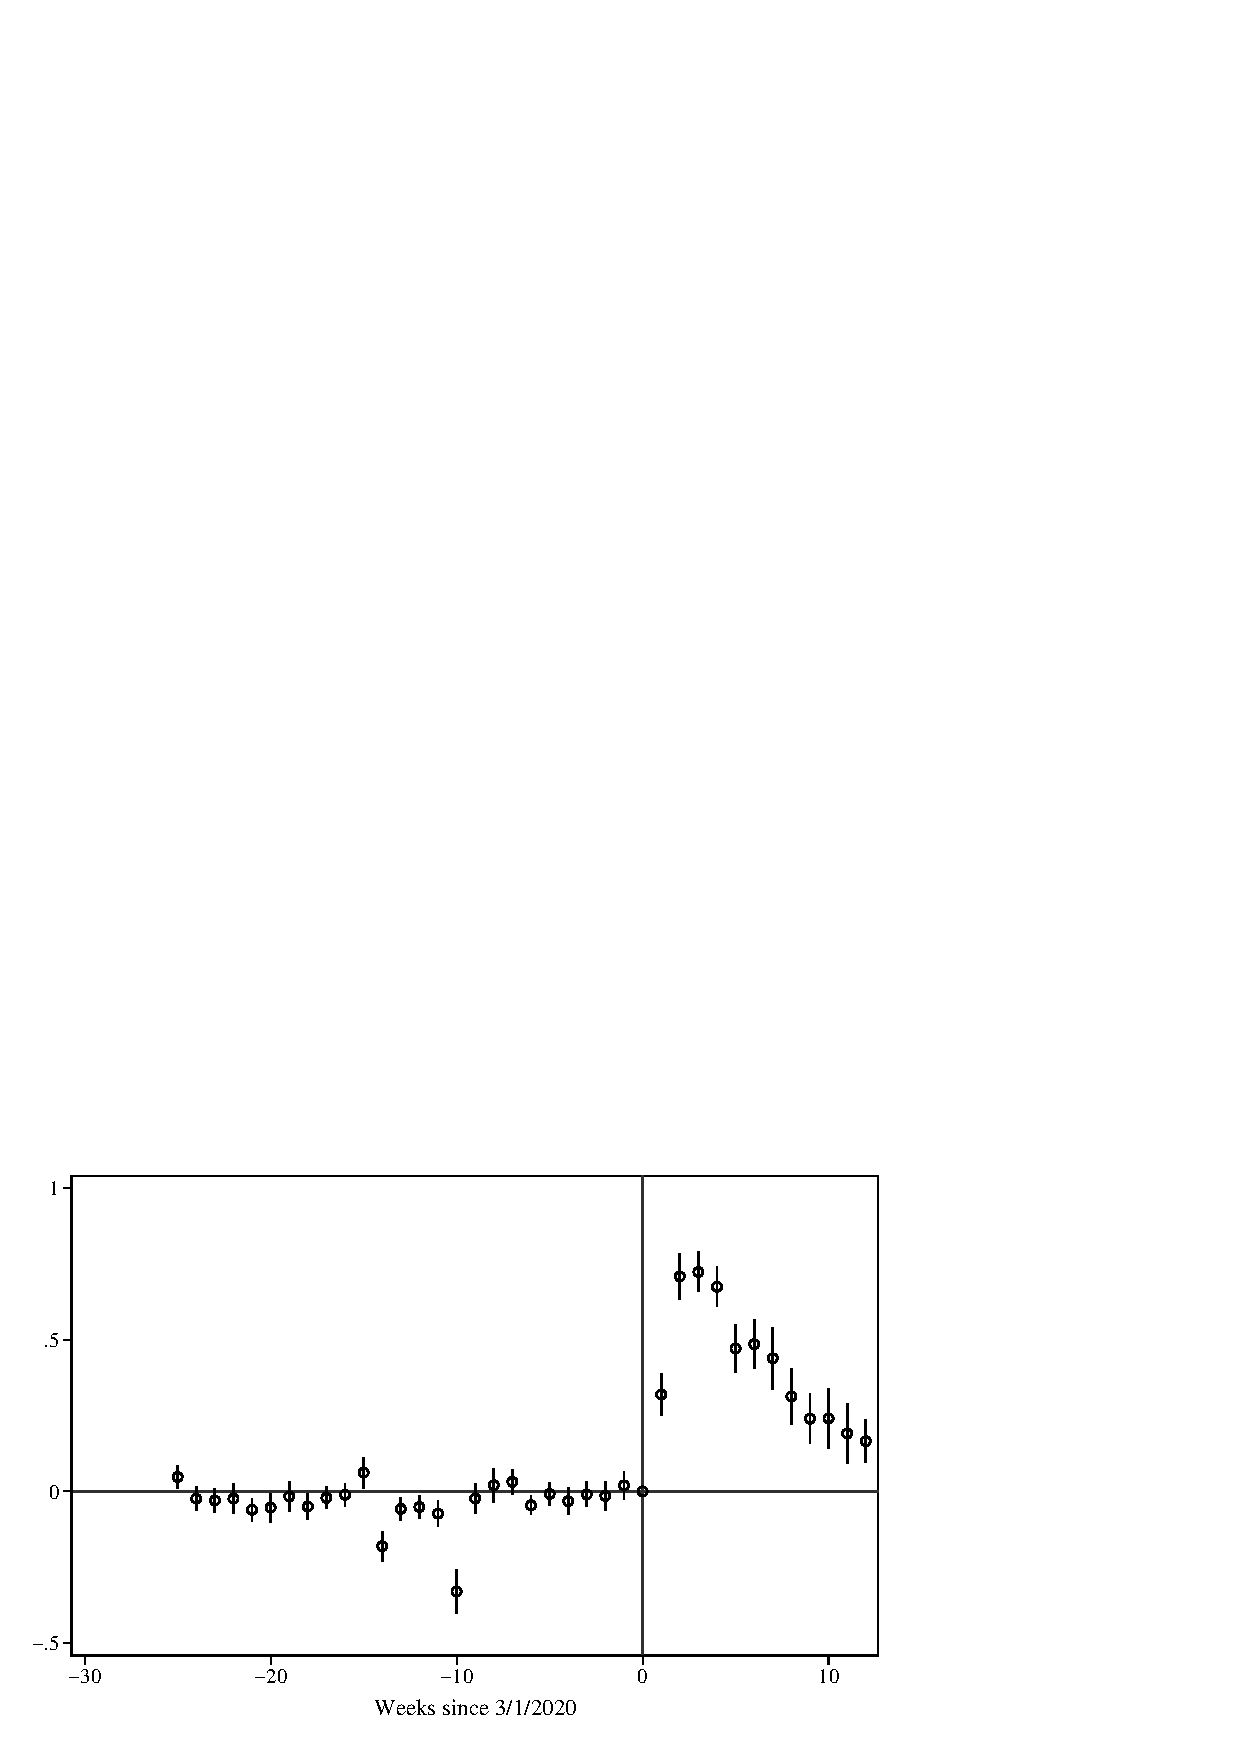
\includegraphics[width=\linewidth]{input/event_study_generic_wks.png}
    \end{subfigure}%
    \begin{subfigure}[t]{0.45\textwidth}
    \caption{Income}
        \centering
        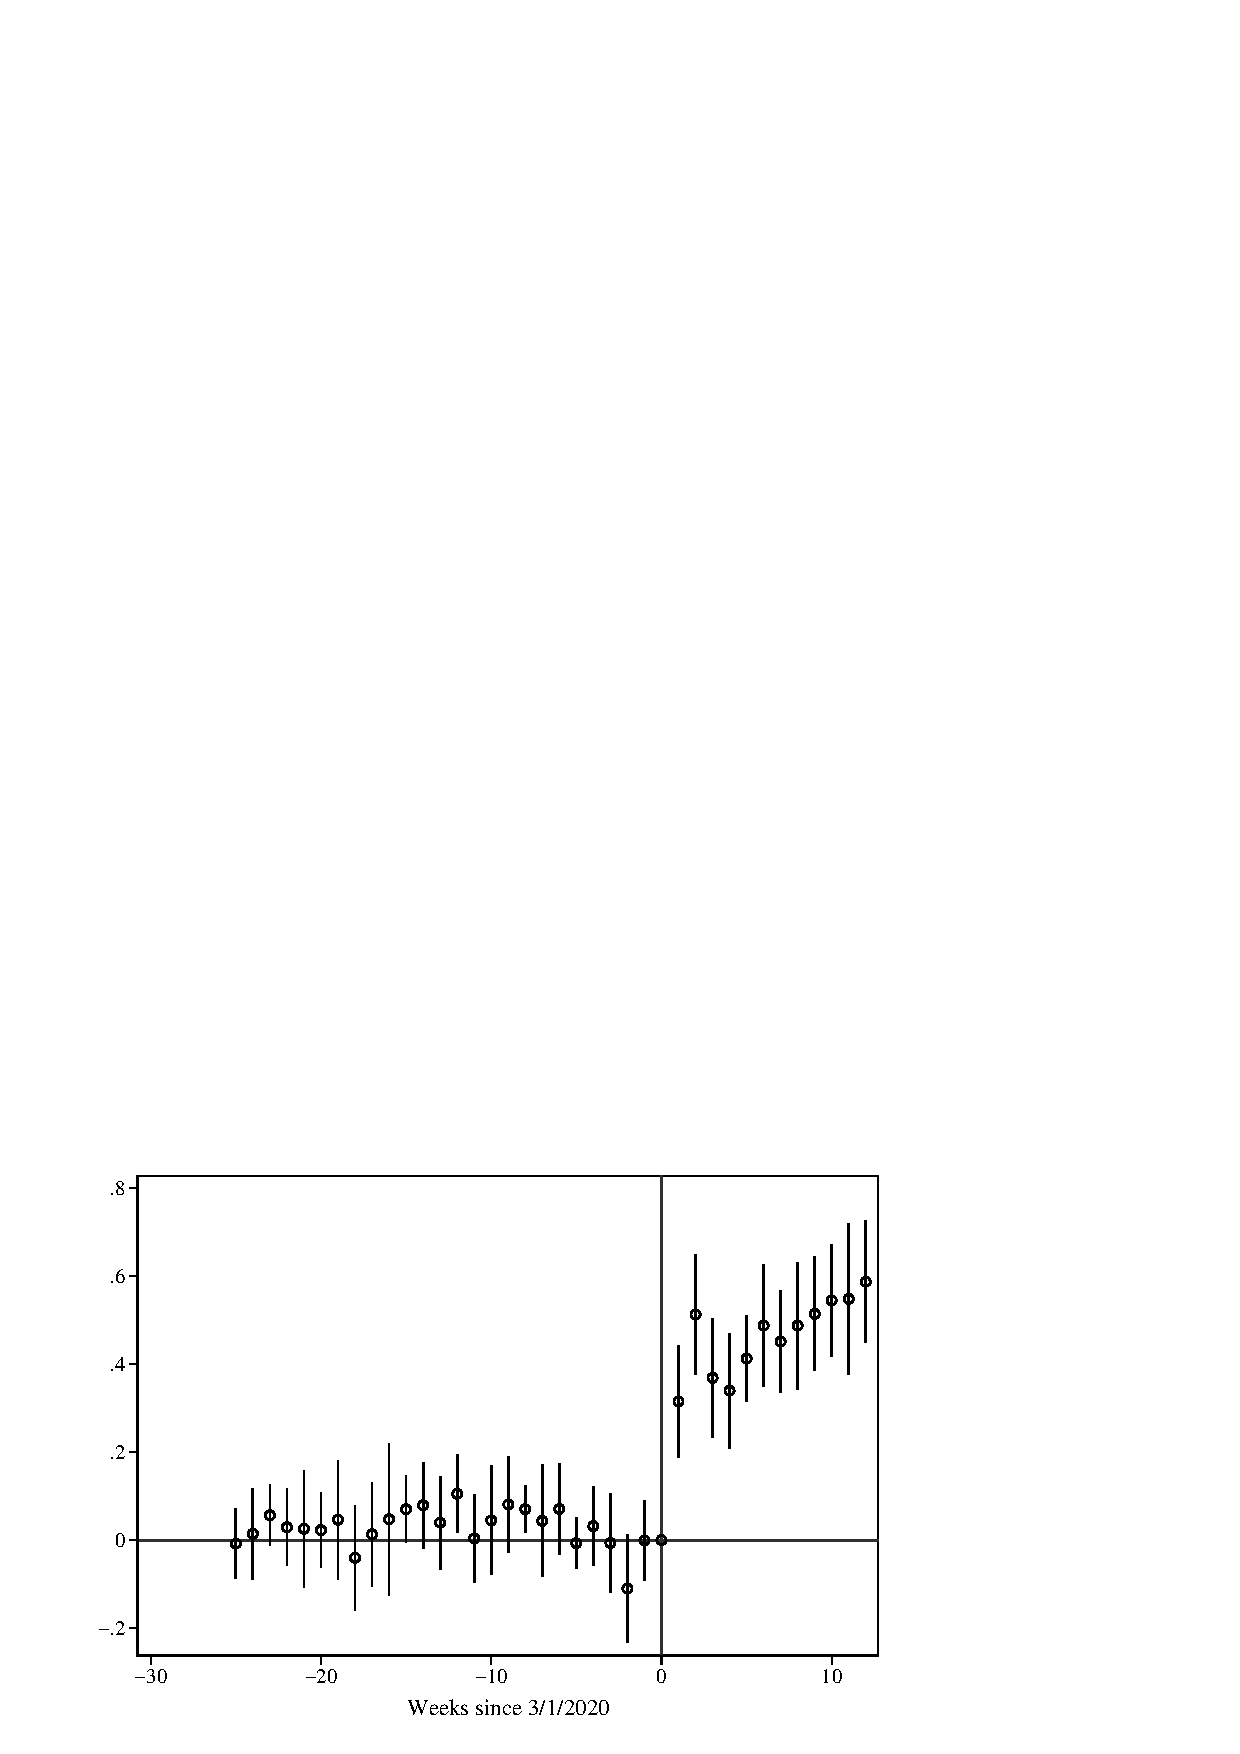
\includegraphics[width=\linewidth]{input/event_study_generic_inc.png}
    \end{subfigure}%

    \begin{subfigure}[t]{0.45\textwidth}
    \caption{Teleworkability}
        \centering
        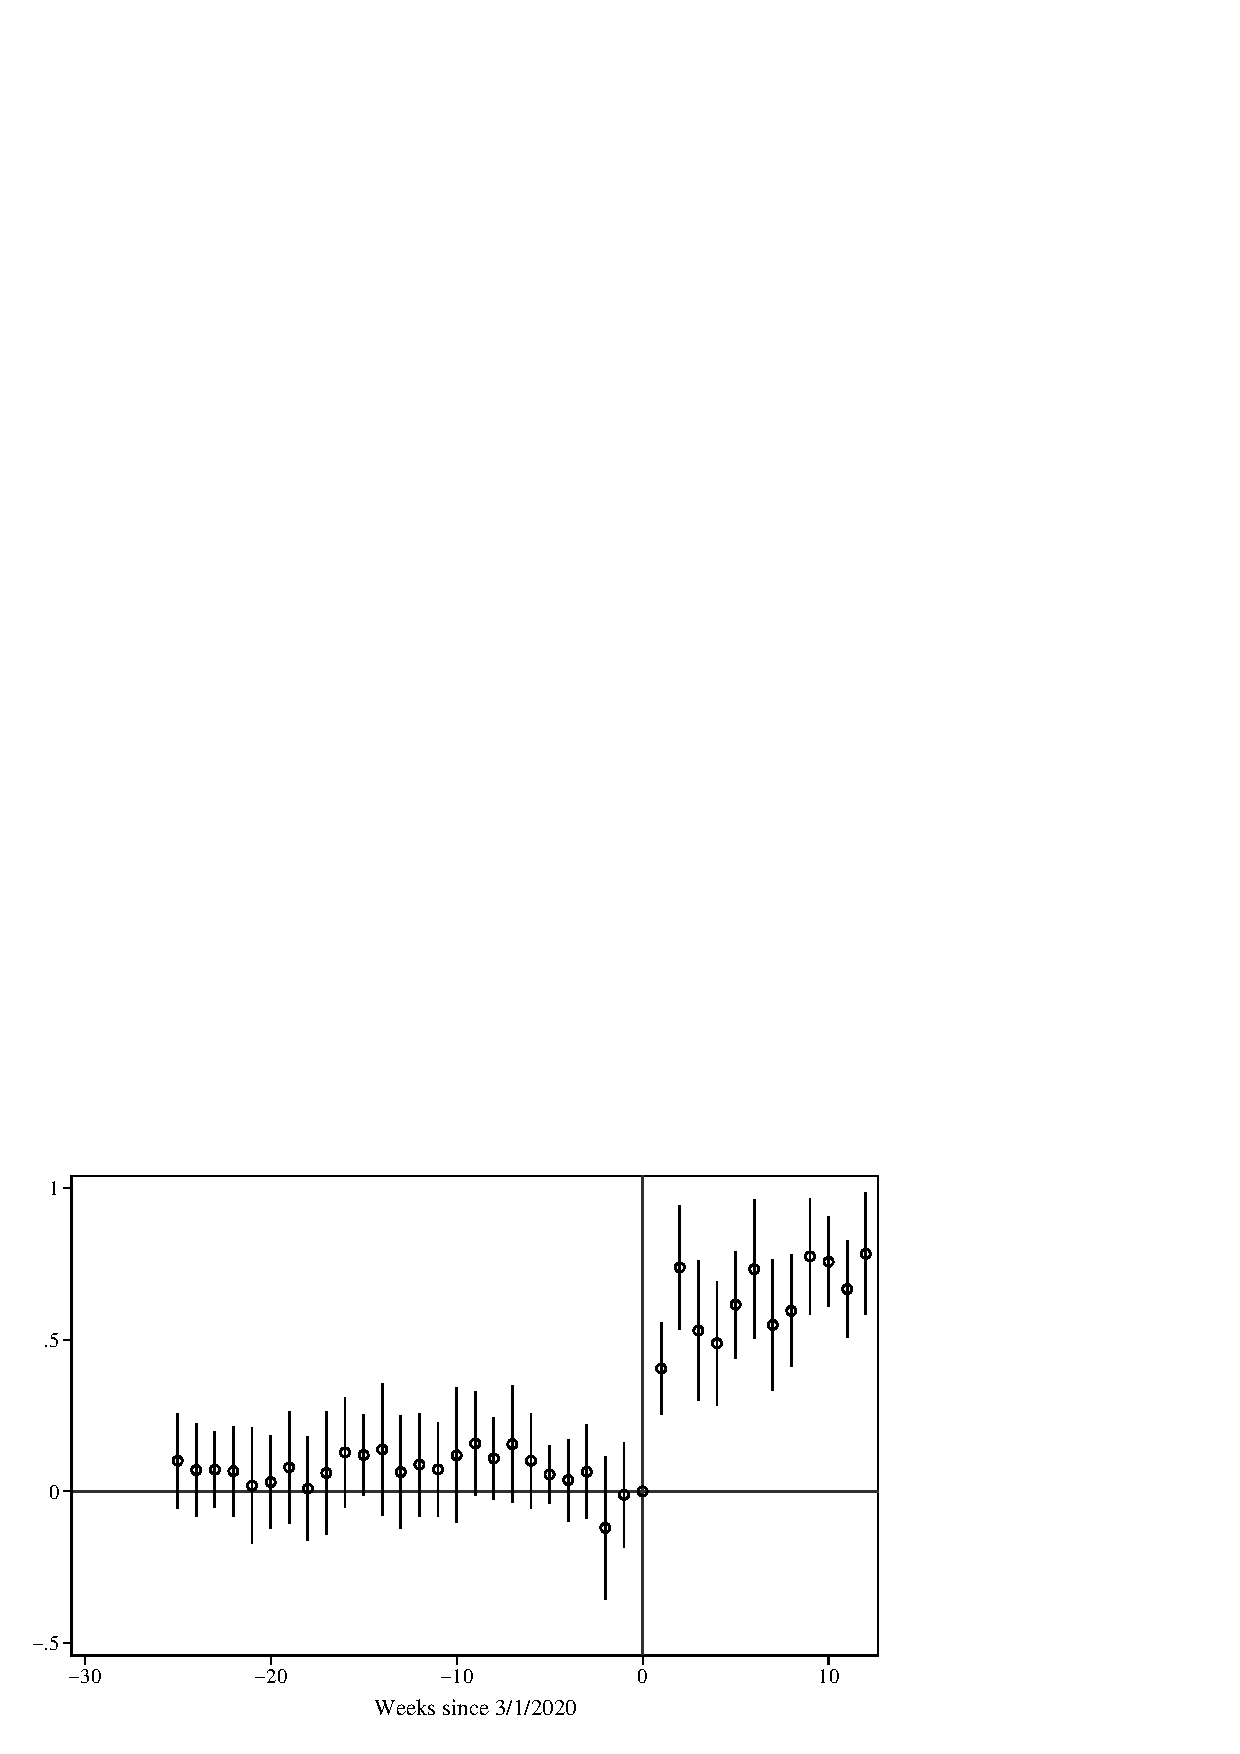
\includegraphics[width=\linewidth]{input/event_study_generic_tele.png}
    \end{subfigure}%
    \begin{subfigure}[t]{0.45\textwidth}
    \caption{Income + Teleworkability}
        \centering
        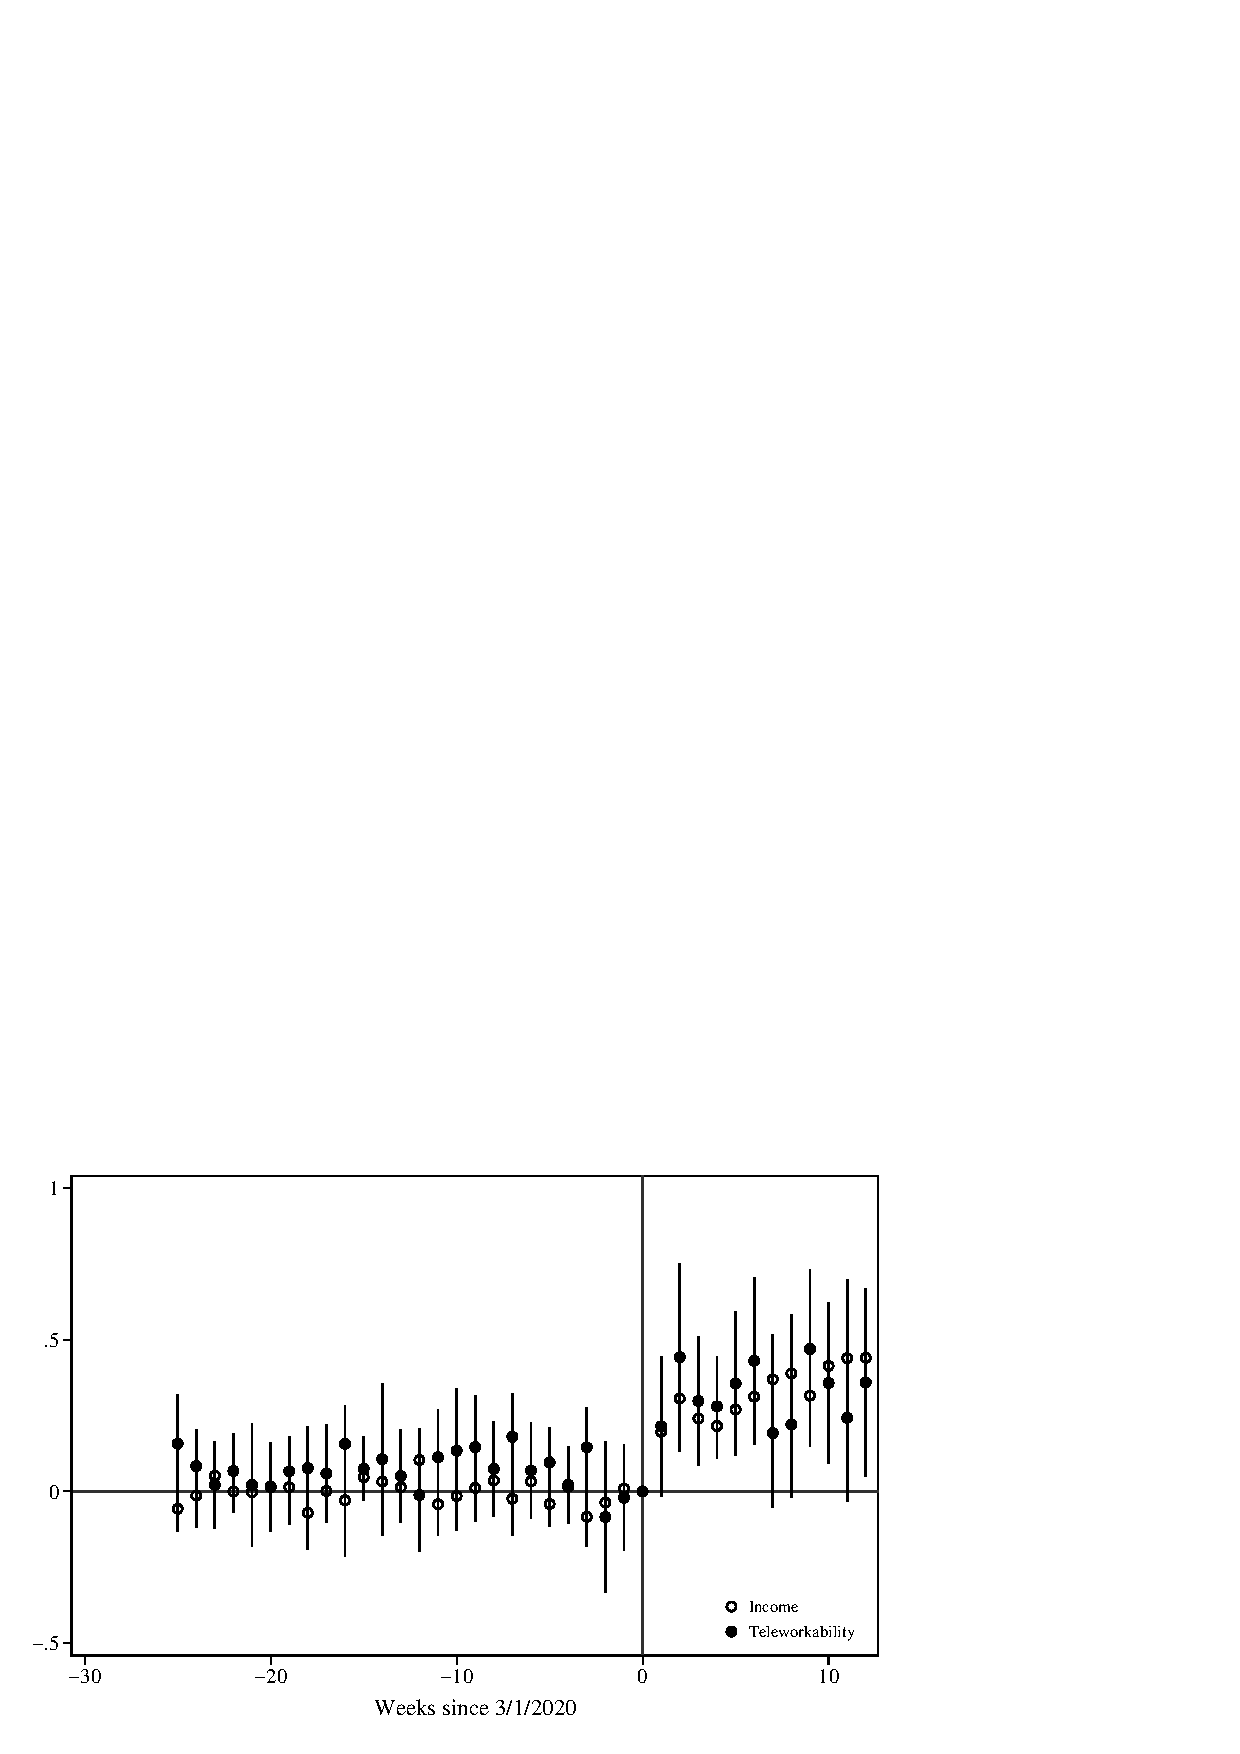
\includegraphics[width=\linewidth]{input/event_study_generic_inctele.png}
    \end{subfigure}%
\end{figure}


\begin{figure}
  \caption{Engagement}
    \centering
    \begin{subfigure}[t]{0.45\textwidth}
    \caption{Intensity}
        \centering
        \includegraphics[width=\linewidth]{input/event_study_engagement_wks.png}
    \end{subfigure}%
    \begin{subfigure}[t]{0.45\textwidth}
    \caption{Income}
        \centering
        \includegraphics[width=\linewidth]{input/event_study_engagement_inc.png}
    \end{subfigure}%

    \begin{subfigure}[t]{0.45\textwidth}
    \caption{Teleworkability}
        \centering
        \includegraphics[width=\linewidth]{input/event_study_engagement_tele.png}
    \end{subfigure}%
    \begin{subfigure}[t]{0.45\textwidth}
    \caption{Income + Teleworkability}
        \centering
        \includegraphics[width=\linewidth]{input/event_study_engagement_inctele.png}
    \end{subfigure}%

  \caption{Badges}
    \centering
    \begin{subfigure}[t]{0.45\textwidth}
    \caption{Intensity}
        \centering
        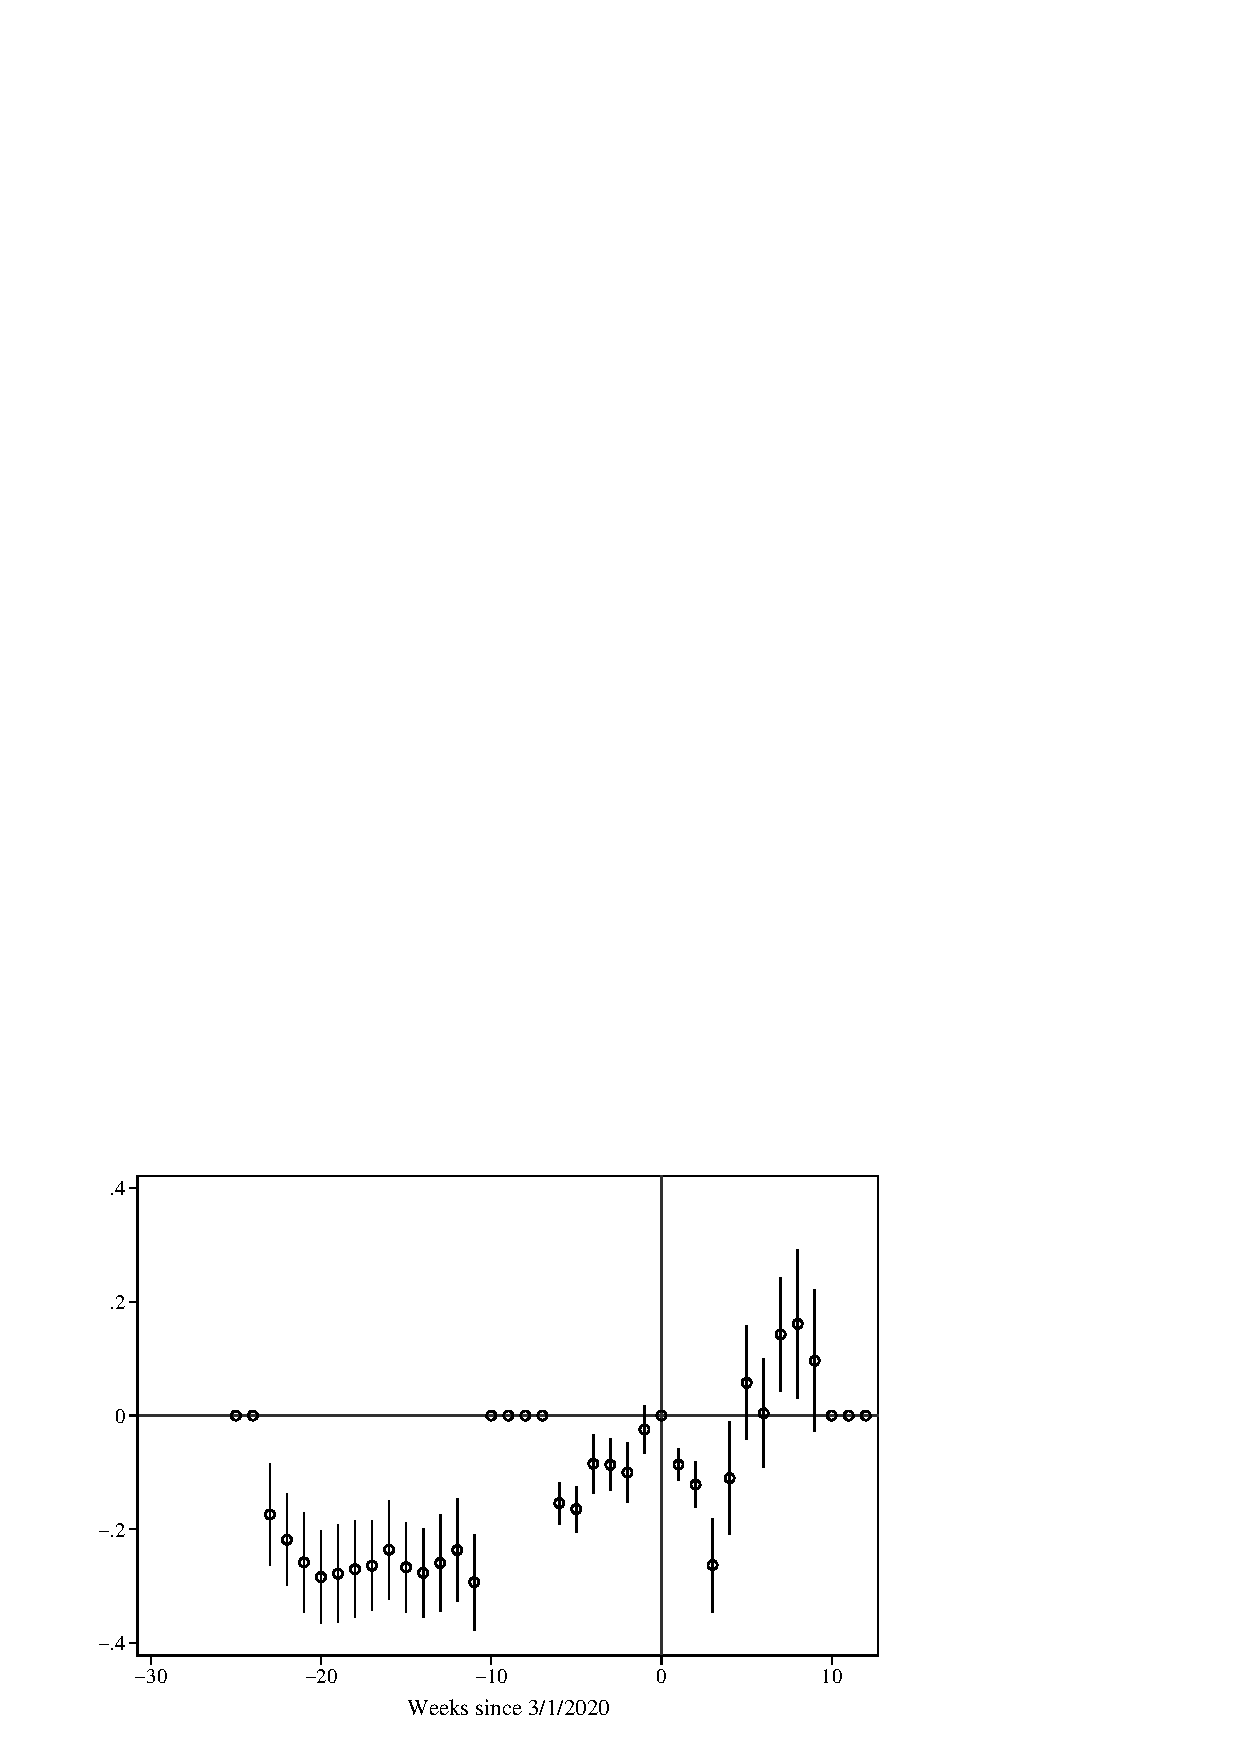
\includegraphics[width=\linewidth]{input/event_study_badges_wks.png}
    \end{subfigure}%
    \begin{subfigure}[t]{0.45\textwidth}
    \caption{Income}
        \centering
        \includegraphics[width=\linewidth]{input/event_study_badges_inc.png}
    \end{subfigure}%

    \begin{subfigure}[t]{0.45\textwidth}
    \caption{Teleworkability}
        \centering
        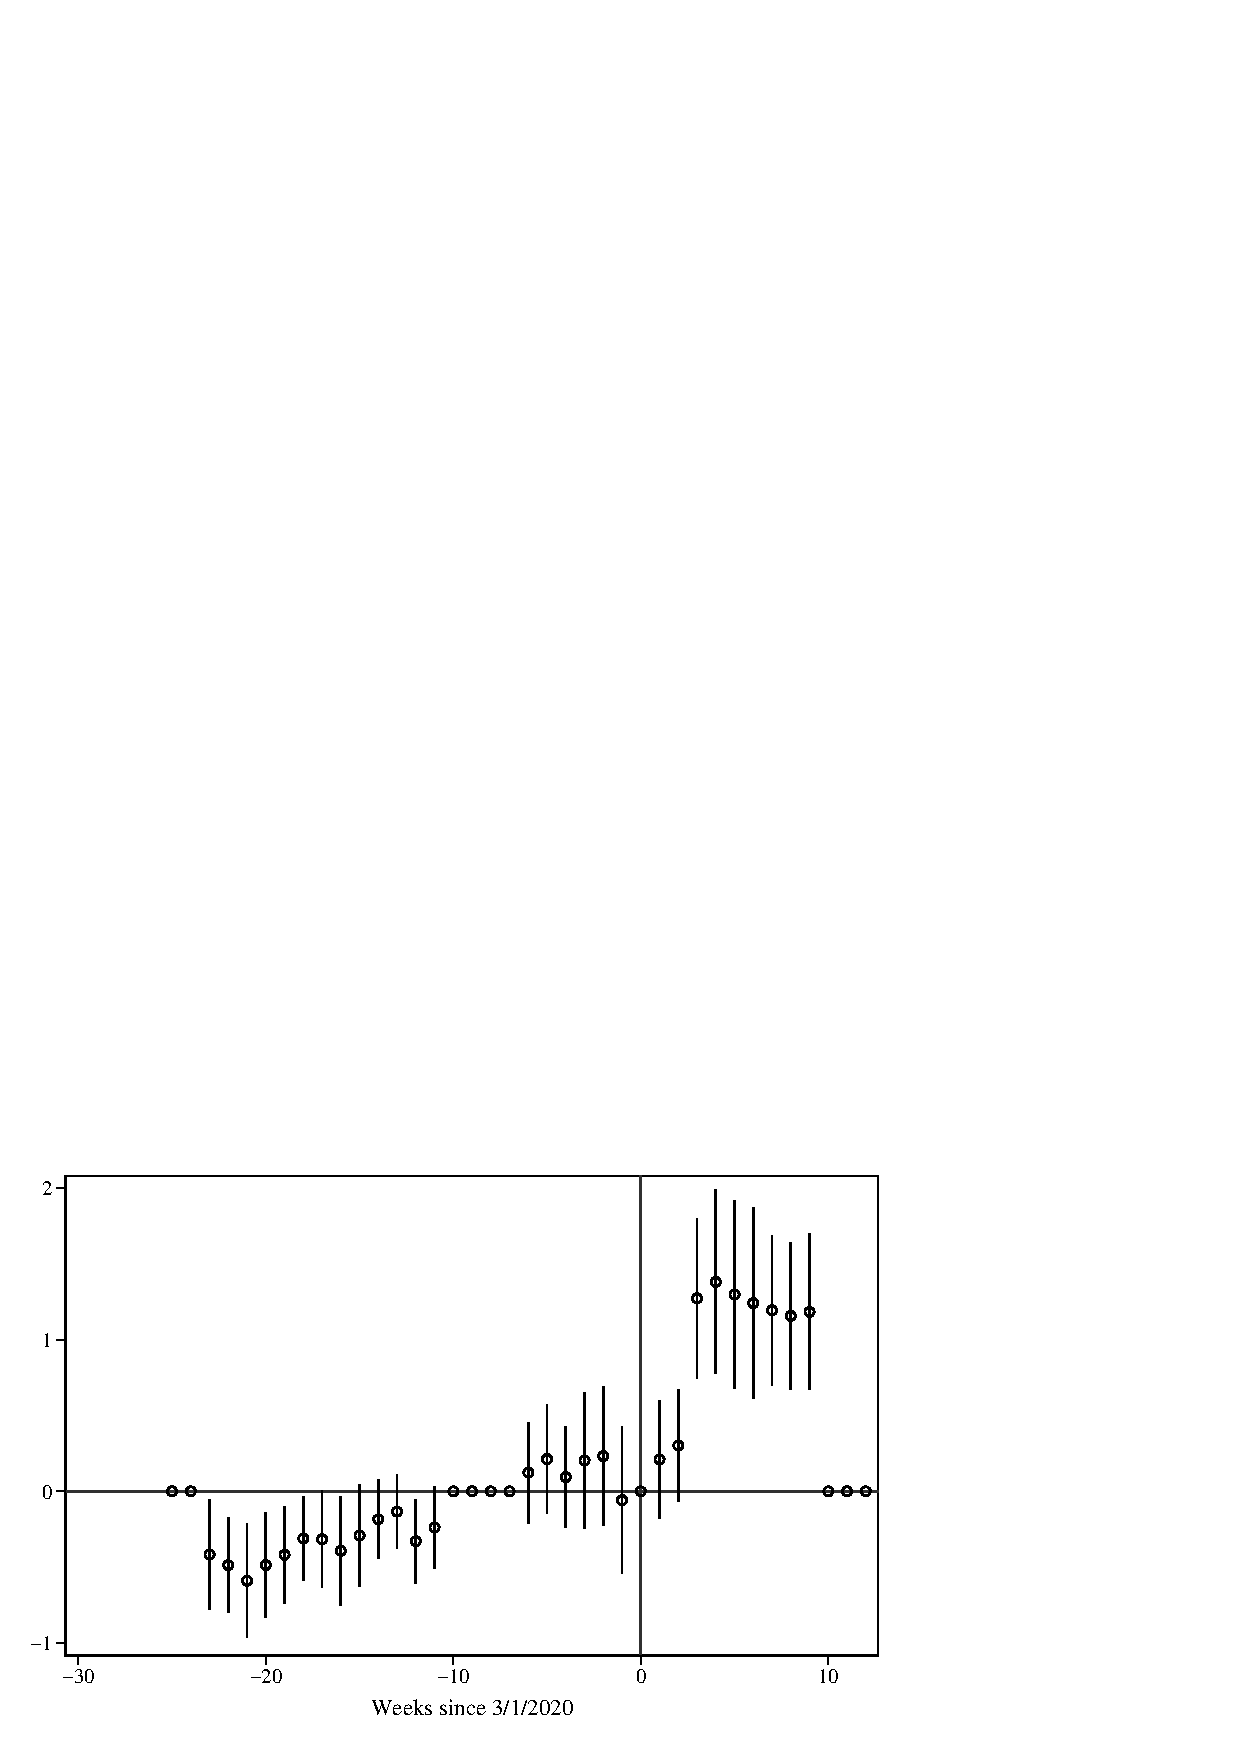
\includegraphics[width=\linewidth]{input/event_study_badges_tele.png}
    \end{subfigure}%
    \begin{subfigure}[t]{0.45\textwidth}
    \caption{Income + Teleworkability}
        \centering
        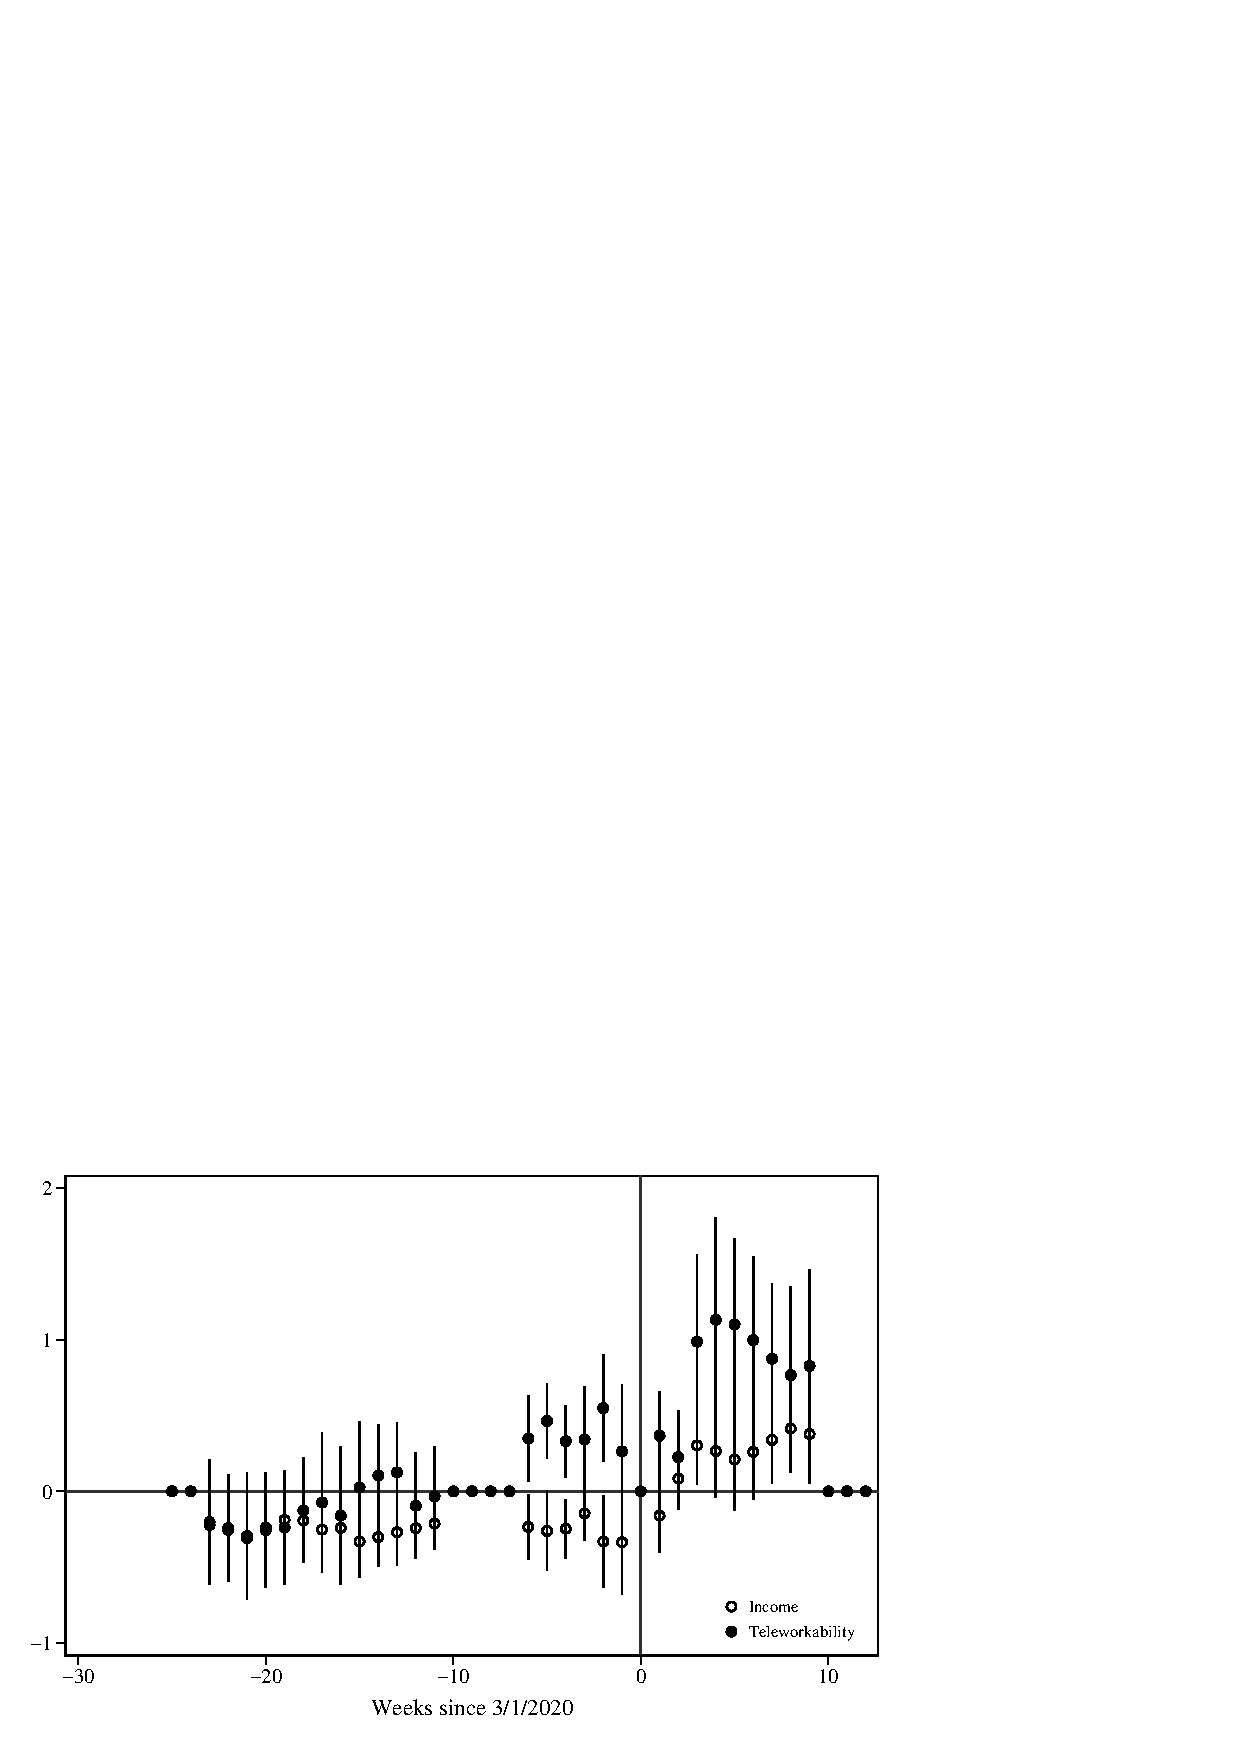
\includegraphics[width=\linewidth]{input/event_study_badges_inctele.png}
    \end{subfigure}%
\end{figure}
   
% %%LOGBOOK ENTRIES: Related literature
% \chapter{Notes on related literature}
%
% %%LOGBOOK ENTRIES: Research design
% \chapter{Research design}
%
% %%LOGBOOK ENTRIES: Data description
% \chapter{Data description}
%
%
% %%LOGBOOK ENTRIES: FEEDBACK
% \chapter{Feedback}
%
%
% %%LOGBOOK ENTRIES: FAQ
% \chapter{Frequently asked questions}

%%LOGBOOK BIBLIOGRAPHY


%%NON-CHRONOLOGICAL ENTRIES
\chapter{Research infrastructure (from Jonathan Dingel)}
\input{entries/researchinfrastructure.tex}

\section{Task-based organization of code and data} \input{entries/tasks.tex}
\section{Writing code} \input{entries/codestylesheet.tex}
\section{Running code with Make} \input{entries/make.tex}
\section{Tracking code with Git} \input{entries/git_alone.tex}

\section{Sharing code via Git} \input{entries/git_together.tex}
\section{Sharing results via the logbook} \input{entries/logbookexplained.tex}

\section{Unix/Linux shell commands} \input{entries/unixshelltips.tex}
\section{Aesthetics and visualization} \input{entries/visualization.tex}
\section{Manuscript preparation} \input{entries/manuscriptpreparation.tex}
\section{Notes on Julia} \input{entries/juliaintro.tex}

\section{Notes on Stata} \input{entries/statanotes.tex}


\end{document}
